\documentclass[12pt,a4paper,oneside]{report}
\usepackage[T1]{fontenc}
\usepackage{mathptmx}
\usepackage[left=30mm,right=25mm,top=25mm,bottom=25mm]{geometry}

\usepackage{titlesec}
\usepackage{fancyhdr}
\setlength{\headheight}{30pt}
\setlength{\headsep}{12pt}

\usepackage{amsmath,amssymb}
\usepackage{booktabs,tabularx,multirow}
\usepackage{xcolor}
\usepackage{tikz}
\usetikzlibrary{arrows.meta,positioning,fit,calc,backgrounds}
\usepackage[font=small,labelfont=bf]{caption}
\usepackage{microtype}
\usepackage{graphicx,array,longtable,pdflscape,setspace}
\usepackage[hidelinks]{hyperref}
\onehalfspacing
\setlength{\parindent}{0pt}
\setlength{\parskip}{4pt}
\setcounter{tocdepth}{1}
\renewcommand{\contentsname}{Table of Contents}
\newcommand{\institutionlogo}[1]{\IfFileExists{amrita-logo.png}{
\includegraphics[width=#1]{amrita-logo.png}}{\fbox{\parbox{#1}{\centering Amrita Vishwa Vidyapeetham\\Place amrita-logo.png beside this file}}}}
\graphicspath{{figures/}}

\newcommand{\ProjectTitle}{Runtime Computational Memory: Understanding Emergent Behaviour through KV-Cache Dynamics in Transformer Language Models}
\newcommand{\GuideName}{Dr. Thara Shyam}
\newcommand{\GuideLine}{Department of Computer Science and Engineering}
\newcommand{\CoordinatorName}{Dr. Divya Udayan J}
% Fill in before printing; a blank signature line is printed until then.
\newcommand{\ChairpersonName}{\rule{0.36\textwidth}{0.4pt}}
\newcommand{\ReportDate}{October 2026}
\newcommand{\StudentA}{S Kunal Achintya Reddy}\newcommand{\RegA}{AM.SC.U4CSE23352}
\newcommand{\StudentB}{V Sriman Vashishta}\newcommand{\RegB}{AM.SC.U4CSE23368}
\newcommand{\StudentC}{Raaghavan M S}\newcommand{\RegC}{AM.SC.U4CSE23330}
\newcommand{\StudentD}{B Nithilesh}\newcommand{\RegD}{AM.SC.U4CSE23311}

\fancypagestyle{project}{%
  \fancyhf{}
  \fancyhead[C]{\parbox{\textwidth}{\centering\small\nouppercase{\ProjectTitle}}}
  \fancyfoot[C]{\thepage}
  \renewcommand{\headrulewidth}{0.4pt}
}
% Preliminary pages show only a page number.
\fancypagestyle{plain}{%
  \fancyhf{}
  \fancyfoot[C]{\thepage}
  \renewcommand{\headrulewidth}{0pt}
}
\newcommand{\EnableProjectHeaders}{%
  \pagestyle{project}%
  % report uses plain style on chapter-opening pages.
  \fancypagestyle{plain}{%
    \fancyhf{}
    \fancyhead[C]{\parbox{\textwidth}{\centering\small\nouppercase{\ProjectTitle}}}
    \fancyfoot[C]{\thepage}
    \renewcommand{\headrulewidth}{0.4pt}
  }%
}
\titlespacing*{\chapter}{0pt}{0pt}{16pt}
\titlespacing*{\section}{0pt}{10pt}{4pt}
\titlespacing*{\subsection}{0pt}{8pt}{3pt}
\titlespacing*{\subsubsection}{0pt}{6pt}{3pt}
\raggedbottom

% table helpers
\newcolumntype{L}[1]{>{\raggedright\arraybackslash}p{#1}}
\newcolumntype{Y}{>{\raggedright\arraybackslash}X}
\renewcommand{\arraystretch}{1.2}

\begin{document}
\pagestyle{empty}

{\centering \Large\bfseries \ProjectTitle{}\par}
\vspace{10pt}
{\centering Project report submitted in partial fulfilment of the requirements for the award of the degree of\par}
\vspace{6pt}
{\centering \textbf{BACHELOR OF TECHNOLOGY}\par}
{\centering in\par}
{\centering \textbf{COMPUTER SCIENCE AND ENGINEERING}\par}
\vspace{8pt}
{\centering Submitted by\par}
\vspace{4pt}
{\centering \fontsize{14}{18}\selectfont
\StudentA{} \quad \RegA\par}

{\centering \fontsize{14}{18}\selectfont
\StudentB{} \quad \RegB\par}

{\centering \fontsize{14}{18}\selectfont
\StudentC{} \quad \RegC\par}

{\centering \fontsize{14}{18}\selectfont
\StudentD{} \quad \RegD\par}
\vspace{8pt}
{\centering \fontsize{14}{18}\selectfont
Under the guidance of\par
\GuideName\par
\GuideLine\par}
\vspace{8pt}
{\centering \institutionlogo{4.5in}\par}
\vspace{4pt}
{\centering \textbf{AMRITA SCHOOL OF COMPUTING}\par}
{\centering \textbf{AMRITA VISHWA VIDYAPEETHAM}\par}
{\centering \textbf{AMRITAPURI CAMPUS}\par}
{\centering \textbf{KOLLAM 690525}\par}
{\centering \textbf{OCTOBER 2026}\par}


\clearpage
{\centering \institutionlogo{3.7in}\par}
\vspace{6pt}
{\centering \textbf{DEPARTMENT OF COMPUTER SCIENCE AND ENGINEERING}\par}
{\centering Amrita School of Computing, Amritapuri Campus\par}
\vspace{10pt}
{\centering \Large\bfseries BONAFIDE CERTIFICATE\par}
\vspace{10pt}
\begin{sloppypar}
This is to certify that the project report entitled ``\ProjectTitle{}'', submitted by \StudentA{} (\RegA), \StudentB{} (\RegB), \StudentC{} (\RegC) and \StudentD{} (\RegD), in partial fulfilment of the requirements for the award of the degree of Bachelor of Technology in Computer Science and Engineering at Amrita Vishwa Vidyapeetham, is a bonafide record of the work carried out by them under my guidance and supervision at Amrita School of Computing, Amritapuri, during Semester 7 of the academic year 2026--2027.
\end{sloppypar}

\vspace{24pt}
\begin{tabular}{p{.46\textwidth}p{.46\textwidth}} \GuideName & \CoordinatorName \\ Project Guide & Project Coordinator \\[18pt] Signature \hrulefill & Signature \hrulefill \\[30pt] \ChairpersonName &  \\ Chairperson, CSE & Reviewers \\[18pt] Signature \hrulefill & Signature \hrulefill \end{tabular}

\vspace{24pt}
Place: Amritapuri\\
Date: \ReportDate
\clearpage
\thispagestyle{empty}

{\centering
\institutionlogo{3.0in}\par
\vspace{0.2cm}
\textbf{DEPARTMENT OF COMPUTER SCIENCE AND ENGINEERING}\par
Amrita School of Computing, Amritapuri Campus\par
\vspace{0.4cm}
{\Large\bfseries DECLARATION\par}
}

\vspace{0.3cm}

\begin{sloppypar}\setlength{\rightskip}{0pt plus 2em}\noindent
We, \StudentA{} (\RegA), \StudentB{} (\RegB), \StudentC{} (\RegC) and \StudentD{} (\RegD),
hereby declare that the project entitled
``\ProjectTitle{}'' is a record of our original work
carried out under the guidance of \GuideName, \GuideLine,
Amrita Vishwa Vidyapeetham, Amritapuri.
To the best of our knowledge, this work has not formed the
basis for the award of any degree, diploma, fellowship or
similar qualification to any candidate at any university.
All sources and contributions of others have been
appropriately acknowledged.
\end{sloppypar}

\vspace{0.5cm}

\noindent
Place: Amritapuri\\
Date: \ReportDate

\vspace{0.7cm}

\noindent
\begin{tabular}{@{}p{0.60\textwidth}p{0.34\textwidth}@{}}
\textbf{Student details} & \textbf{Signature of the student} \\[8pt]
\StudentA\newline \RegA & \rule{0.30\textwidth}{0.4pt} \\[10pt]
\StudentB\newline \RegB & \rule{0.30\textwidth}{0.4pt} \\[10pt]
\StudentC\newline \RegC & \rule{0.30\textwidth}{0.4pt} \\[10pt]
\StudentD\newline \RegD & \rule{0.30\textwidth}{0.4pt}
\end{tabular}

\vspace{0.5cm}

\noindent
\textbf{Project Guide:} \GuideName

\vspace{0.5cm}

\noindent
\textbf{Signature of the Project Guide:}
\rule{4cm}{0.4pt}

\clearpage
\pagenumbering{roman}
\pagestyle{plain}

\phantomsection
\addcontentsline{toc}{chapter}{Acknowledgement}
{\centering \Large\bfseries ACKNOWLEDGEMENT\par}
\vspace{10pt}
We express our sincere gratitude to our project guide, \GuideName, Department of Computer Science and Engineering, for her continuous guidance throughout this project. Her insistence that every claim be backed by a measurable test, and that a negative result be reported as carefully as a positive one, shaped both the experimental design and the way the findings in this report are presented. Her regular reviews of our design documents, intermediate results and drafts helped us keep the scope realistic for the hardware available to us.

We thank our Project Coordinator, \CoordinatorName, for organising the review schedule and for the feedback received during the design and mid-term reviews, which led directly to clearer objectives and a stricter evaluation plan. We are grateful to the Chairperson and the faculty of the Department of Computer Science and Engineering, and to the reviewers of our earlier submissions, whose questions about attention sinks, negative controls and the relevance of the work to society improved this report.

We thank Amrita School of Computing, Amritapuri, and Amrita Vishwa Vidyapeetham for providing the academic environment and resources that made this work possible. We also acknowledge the open-source community behind PyTorch, Hugging Face Transformers and the Qwen model family, whose publicly available tools and model weights allowed us to study a real language model on a student laptop. Finally, we thank our families and friends for their patience and encouragement during this semester.

\clearpage
\phantomsection
\addcontentsline{toc}{chapter}{Abstract}
{\centering \Large\bfseries ABSTRACT\par}
\vspace{10pt}
Large language models increasingly support hiring, education, healthcare and public services, and they are beginning to work in teams in which one model passes information to another. Social bias in such systems falls mostly on groups that are already disadvantaged, which is the concern of Sustainable Development Goal~10, \emph{Reduced Inequalities}; the project also supports SDG~9, \emph{Industry, Innovation and Infrastructure}, and SDG~16, \emph{Peace, Justice and Strong Institutions}, through open and auditable AI tools. Bias mitigation today mostly requires retraining, while the key--value (KV) cache, the runtime memory a transformer builds during a conversation, is studied only as an efficiency problem. This project treats the KV cache as an object that can be measured and edited. We built an open Python framework that stamps every cache entry with its layer, head, position, turn, agent and source; detects persistent memory attractors; localises bias reservoirs with cross-validated probes; separates bias carried by shared memory from bias carried by text between two agents; and tests cache-only interventions by seed-matched replay against negative controls and a coherence budget. It was evaluated on 135 two-agent conversations with a controlled reference transformer and 135 with the public Qwen2.5-0.5B-Instruct model on a 4~GB laptop GPU, using fictional social groups. In the reference model, shared cache entries left the receiving agent more biased than exchanged text (memory contagion $+0.186$, 95\% interval $+0.034$ to $+0.340$, Mann--Whitney $p = 0.085$), and middle-layer heads predicted bias with AUC up to 0.92; ablating their entries removed 20.3\% of the bias but cost 6.7 points of factual accuracy, so the pre-registered rule rejected it. In Qwen2.5 the bias spread equally through text and memory, and no attractors beyond attention sinks appeared. A public website presents the experiment to non-specialists.

\vspace{6pt}
\textbf{Keywords:} KV cache; large language models; social bias; multi-agent systems; mechanistic interpretability; causal intervention

\clearpage
\tableofcontents
\clearpage
\phantomsection
\addcontentsline{toc}{chapter}{List of Figures}
\listoffigures
\clearpage
\phantomsection
\addcontentsline{toc}{chapter}{List of Tables}
\listoftables
\clearpage
\phantomsection
\addcontentsline{toc}{chapter}{List of Abbreviations}
{\centering \Large\bfseries LIST OF ABBREVIATIONS\par}
\vspace{10pt}
\begin{tabular}{@{}L{0.18\textwidth}L{0.74\textwidth}@{}}
ACE & Average Causal Effect \\
AIC / BIC & Akaike / Bayesian Information Criterion \\
API & Application Programming Interface \\
AUC & Area Under the Receiver Operating Characteristic Curve \\
BBQ & Bias Benchmark for Question Answering \\
BH-FDR & Benjamini--Hochberg False Discovery Rate \\
CI & Confidence Interval \\
CPU / GPU & Central / Graphics Processing Unit \\
FR / NFR & Functional / Non-Functional Requirement \\
GQA & Grouped-Query Attention \\
KV & Key--Value \\
LLM & Large Language Model \\
MC / TC & Memory Contagion / Text Contagion \\
PPL & Perplexity \\
RoPE & Rotary Position Embedding \\
SDG & Sustainable Development Goal \\
TE & Transfer Entropy \\
\end{tabular}

\clearpage
\pagenumbering{arabic}
\pagestyle{plain}
\EnableProjectHeaders

\chapter{Introduction}
\section{Background and motivation}
Transformer language models generate text one token at a time. Before producing each new token, every attention layer compares the current position with all earlier positions of the conversation~\cite{vaswani2017attention}. To avoid recomputing the representations of earlier tokens at every step, the model stores, for every layer and attention head, a \emph{key} vector and a \emph{value} vector for each token it has processed. This growing store is the key--value (KV) cache. It is created during a conversation, it changes with every token that is read or written, and it is discarded when the conversation ends, while the trained weights of the model never change. In that sense the KV cache is the short-term, runtime memory of the model: everything the model ``remembers'' about the current conversation is held there.

Research on the KV cache has so far concentrated on its cost. Long conversations make the cache large, so a substantial body of work studies how to evict, compress, stream or share it efficiently~\cite{xiao2024sinks,zhang2023h2o,liu2023scissorhands,oren2024msrnn,kwon2023vllm}. Several of these studies observe that the cache is highly structured: a few early ``attention sink'' tokens receive large attention regardless of their meaning~\cite{xiao2024sinks}, and a small set of ``heavy-hitter'' entries dominates attention throughout generation~\cite{zhang2023h2o}. However, these structures are studied only to decide which entries can be safely discarded. Whether the information held in the cache shapes what the model \emph{believes} during a conversation, and in particular whether it carries and amplifies social bias, has not been examined.

The question has become practical because language models now work in teams. Multi-agent frameworks let one model search, another write and a third check the result~\cite{wu2023autogen,du2024debate}, and serving systems already reuse cached keys and values across requests to save computation~\cite{kwon2023vllm,yao2025cacheblend}. When agents exchange text, a human can in principle read what was said. When they exchange cache entries, the transferred information is a set of numerical vectors that no person can read. If a one-sided idea can travel from one agent to another through such shared memory, it could spread through an AI system without leaving any visible trace in the exchanged text. A recent survey of bias and fairness in language models~\cite{gallegos2024bias} shows that most mitigation methods act before or during training, which is expensive and out of reach for small institutions, and that few methods act on the model at inference time.

\textbf{Relevance to the Sustainable Development Goals.} The project was proposed under United Nations Sustainable Development Goal~10, \emph{Reduced Inequalities}~\cite{un2015agenda}. Language models are increasingly used to shortlist job applicants, answer health questions, give educational feedback and run public-service chatbots. When these systems carry social bias, the harm falls mostly on groups that are already disadvantaged by gender, religion, disability, origin or economic status. This directly concerns Target~10.2, which calls for the social, economic and political inclusion of all people irrespective of such characteristics, and Target~10.3, which calls for equal opportunity and the elimination of discriminatory practices. The project contributes by making it possible to observe where bias is held inside a running model and to test whether it can be removed without retraining, which lowers the cost of auditing for the smaller organisations that most need it. The work also supports two secondary goals. Under SDG~9, \emph{Industry, Innovation and Infrastructure}, and its Target~9.5 on enhancing scientific research and technological capability, it delivers open, reproducible research software that runs on commodity hardware. Under SDG~16, \emph{Peace, Justice and Strong Institutions}, and its Target~16.6 on effective, accountable and transparent institutions, it provides tools for inspecting and documenting the behaviour of automated decision systems. The intended beneficiaries are the people affected by automated decisions, and the researchers, auditors and developers who build or regulate such systems. The contribution demonstrated in this report is a measurement and intervention toolkit evaluated in a controlled setting; its benefit for real deployments is an expected outcome that depends on the larger-scale validation described in Chapter~7.

\section{Objectives}
The project has five objectives, taken from the approved design document and stated here together with the evaluation method and deliverable for each.

The first objective (O1) is to build a runtime-memory instrumentation framework that records every KV cache entry of a frozen language model together with its provenance: layer, attention head, absolute position, conversation turn, agent and source channel. It is evaluated by unit tests that check provenance stamping, cache transplantation and deterministic replay, and its deliverable is an installable Python package with a trace store.

The second objective (O2) is to detect and characterise persistent \emph{memory attractors}, that is, cache entries that keep receiving attention long after they were written, and to separate them from the known attention-sink phenomenon. It is evaluated with four metrics (reuse, lifetime, persistence and centrality) under pre-registered thresholds, and its deliverable is the attractor statistics for every conversation.

The third objective (O3) is to test whether bias is concentrated in identifiable \emph{bias reservoirs}, specific attention heads whose cached values predict the bias of a conversation. It is evaluated by cross-validated probe AUC with false-discovery-rate control and by the measured effect of ablating each head, and its deliverable is a ranked reservoir map.

The fourth objective (O4) is to measure \emph{memory contagion}, the part of bias transfer between two agents that is carried by shared cache entries rather than by exchanged text, and to test whether bias rises abruptly at a critical level of one-sided input (a phase transition). It is evaluated by a three-arm experiment with bootstrap confidence intervals and a Mann--Whitney test, and by comparing logistic and linear fits, and its deliverable is the contagion decomposition and phase analysis.

The fifth objective (O5) is to change behaviour by editing the cache alone. Ablation, perturbation and gating interventions are tested under seed-matched replay against random-head and sink-only negative controls, and an intervention is accepted only if it stays within a coherence budget of at most 5\% perplexity increase and at most 2 points of factual-accuracy loss. Its deliverable is a causal intervention toolkit with the accept or reject decision for each intervention.

\section{Scope and constraints}
The intended users of the framework are researchers, auditors and developers who need to inspect how a language model uses its runtime memory. The project covers decoder-only transformer models whose weights are publicly available, two-agent conversations between instances of the same model, and social bias measured on fictional groups, with factual question answering used as a coherence check. The model weights are never modified: every measurement and every intervention acts only on the KV cache during inference.

Three constraints shaped the work. First, the available hardware was a laptop with a 4~GB NVIDIA GTX 1650~Ti GPU. The design document targets 7--8 billion parameter models such as Llama-3-8B, which need roughly 16~GB of GPU memory for their weights alone. The framework supports these models through configuration files, but in this phase it was evaluated on a controlled reference transformer and on the 0.5 billion parameter Qwen2.5-0.5B-Instruct model~\cite{qwen2024}. Second, to make the direction of bias known by construction and to avoid making statements about real communities, the probes use invented group names such as ``Vorlan'' and ``Tessic'' rather than real demographic groups, following the question formats of established benchmarks~\cite{parrish2022bbq,nadeem2021stereoset,nangia2020crows,lin2022truthfulqa}. Third, cache sharing between agents is only defined for agents running the same base model, because cached keys and values are not portable across tokenizers or architectures. Fine-tuning, retraining and debiasing of weights are outside the scope of the project.

\section{Project report organization}
The rest of this report is organised as follows. Chapter~2 states the problem and analyses the limitations of existing approaches. Chapter~3 reviews twelve research papers on KV cache structure, interpretability and intervention, multi-agent interaction and bias measurement, and compares them in a table. Chapter~4 lists the functional, non-functional, hardware and software requirements. Chapter~5 presents the architecture, the experimental protocol, the metrics and the intervention procedure, together with the demonstration website. Chapter~6 describes the evaluation setup and criteria, reports the results for both models, compares them with existing work and with the expected outcomes of the design document, and discusses limitations. Chapter~7 concludes and lays out the work planned for the next phase. Appendix~A documents how to install, run and verify the software.

\chapter{Problem Definition}
\section{Problem statement}
During a conversation a transformer language model accumulates a KV cache that every later token reads before it is generated. The cache therefore acts as a second state of the model, one that changes during the conversation while the weights stay fixed. The problem addressed in this project is that there is currently no way to observe how this runtime memory evolves over a long, multi-agent conversation, no way to attribute an emergent behaviour such as social bias to identifiable structures inside it, and no tested way to change that behaviour by acting on the memory alone.

The research question is stated as follows. \emph{When one language-model agent is exposed to one-sided information about a group of people and then interacts with a second agent, does the bias reach the second agent; does sharing cache entries carry more of it than exchanging text; is the bias held in identifiable parts of the cache; and can it be reduced by editing the cache without damaging the model's general competence?}

Three groups of stakeholders are affected. People who are evaluated or served by automated systems bear the consequences of biased outputs, and these consequences are unequal across social groups, which links the problem to SDG~10. Developers and operators of multi-agent systems need to know whether optimisations such as cache sharing introduce hidden channels for unwanted information. Auditors and researchers need tools that make the runtime behaviour of models inspectable and that produce reproducible evidence. If the problem is left unaddressed, bias that enters one agent of a system could spread to others through a channel that cannot be read in the conversation transcript, and the only remedies available would remain retraining or fine-tuning, which are costly and opaque.

The system takes as input a frozen open-weight model, a probe that defines a fictional group and a pair of opposing traits, the memory arm (shared cache, text only, or no contact), the semantic pressure~$\pi$ (the fraction of one-sided statements shown to the first agent), a random seed, and optionally an intervention specification. It produces a provenance-stamped trace of every cache entry, the bias index of both agents after every turn, attractor and reservoir analyses across many conversations, the contagion decomposition and phase analysis, and an accept or reject decision for each intervention together with its causal effect and coherence cost.

\section{Existing system and limitations}
Existing work touches each part of this problem but none addresses it end to end. The limitations below are drawn from the papers reviewed in Chapter~3.

\textbf{KV cache efficiency methods treat structure only as a compression signal.} StreamingLLM keeps a few initial tokens because they act as attention sinks~\cite{xiao2024sinks}; H2O keeps heavy-hitter tokens that accumulate the most attention~\cite{zhang2023h2o}; Scissorhands relies on the observation that important tokens stay important~\cite{liu2023scissorhands}; and TOVA treats the cache as the state of a multi-state recurrent network and evicts the least-attended entries~\cite{oren2024msrnn}. These methods show that runtime memory is strongly structured, but they evaluate only perplexity, accuracy and throughput. None asks what information the retained entries carry or how they affect bias, and none records which turn, agent or source produced an entry.

\textbf{Interpretability methods study single forward passes or weights, not evolving memory.} Causal mediation analysis localised gender bias to a small number of attention heads in GPT-2~\cite{vig2020causal}, causal tracing localised factual associations to middle-layer MLP modules~\cite{meng2022rome}, and function vectors showed that a few heads transport a compact representation of an in-context task~\cite{todd2024fv}. These studies analyse one prompt at a time, so they cannot follow how a belief builds up across the turns of a conversation or how it moves between agents.

\textbf{Existing interventions modify weights or activations.} ROME edits weights to change a stored fact~\cite{meng2022rome}, and inference-time intervention shifts the outputs of selected heads to improve truthfulness~\cite{li2023iti}. Neither acts on the cached keys and values of a conversation, and inference-time intervention reports a trade-off between the targeted improvement and general helpfulness, which shows that an intervention must be checked for side effects.

\textbf{Multi-agent studies measure only the exchanged text.} Multi-agent debate shows that agents strongly influence each other's answers~\cite{du2024debate}, but it treats the models as black boxes and does not consider a memory-level channel between them.

\textbf{Bias benchmarks are static and single-turn.} BBQ, StereoSet and CrowS-Pairs measure bias in isolated prompts~\cite{parrish2022bbq,nadeem2021stereoset,nangia2020crows}, and TruthfulQA does the same for falsehoods~\cite{lin2022truthfulqa}. They do not measure how bias accumulates during a conversation, and when real group names are used the measured bias mixes what the model learned in training with what it was told in the conversation.

\textbf{Mitigation is expensive.} The mitigation methods surveyed by Gallegos et al.~\cite{gallegos2024bias} act mostly on training data or training objectives, which requires access to large compute budgets.

The gap addressed by this project is therefore the combination of four missing capabilities: recording the KV cache with full provenance over multi-turn, multi-agent conversations; testing for persistent memory structures beyond attention sinks; separating the memory channel from the text channel when bias spreads between agents; and evaluating cache-only interventions with negative controls and a coherence budget. Table~\ref{tab:gap} summarises how each family of existing work relates to these capabilities.

\begin{table}[htbp]
\centering
\caption{Existing approaches and the gap addressed by this project}\label{tab:gap}
\small
\begin{tabularx}{\textwidth}{@{}L{3.2cm}YY@{}}
\toprule
\textbf{Family of work} & \textbf{What it shows} & \textbf{What it does not provide} \\
\midrule
KV cache compression~\cite{xiao2024sinks,zhang2023h2o,liu2023scissorhands,oren2024msrnn} & The cache has stable, high-attention structure (sinks, heavy hitters, persistent entries). & Any link between cache structure and behaviour; provenance of entries; multi-agent settings. \\
Mechanistic interpretability~\cite{vig2020causal,meng2022rome,todd2024fv} & Bias, facts and tasks can be localised to a few components. & Analysis of memory that evolves across turns and agents. \\
Weight and activation editing~\cite{meng2022rome,li2023iti} & Targeted edits can change behaviour. & Edits restricted to the runtime cache; systematic negative controls. \\
Multi-agent interaction~\cite{du2024debate} & Agents change each other's outputs. & A mechanism below the text level. \\
Bias benchmarks and surveys~\cite{parrish2022bbq,lin2022truthfulqa,gallegos2024bias} & How to measure bias and falsehood; taxonomy of mitigation. & Multi-turn accumulation; inference-time, memory-level mitigation. \\
\bottomrule
\end{tabularx}
\end{table}

\chapter{Literature Review}
\section{Review scope and selection}
The review covers research that bears on four questions raised by the project: how the KV cache is structured during generation, how behaviour can be localised to and changed through specific model components, how language-model agents influence one another, and how social bias and factual reliability are measured. Papers were located through the ACL Anthology, the proceedings of NeurIPS, ICLR and ICML, arXiv and Google Scholar, using the keywords \emph{KV cache}, \emph{attention sink}, \emph{KV cache compression}, \emph{heavy hitter}, \emph{causal mediation analysis}, \emph{model editing}, \emph{inference-time intervention}, \emph{function vectors}, \emph{multi-agent language models}, \emph{social bias benchmark} and \emph{truthfulness}. A paper was selected when it was a primary, peer-reviewed publication from 2020 to 2024, when it proposed a method, dataset or analysis directly reused or contrasted in this project, and when its claims could be checked against the published text. Surveys were admitted only where they define the evaluation and mitigation taxonomy used in the project. Eight of the twelve selected works were already cited in the project's design document; the remaining four were added during implementation because they bear directly on the persistence metric, the bias-localisation method and the intervention design.

The selected works fall into four groups. The first group (Sections~\ref{lit:sinks}--\ref{lit:tova}) studies the structure of the KV cache for efficiency. The second group (Sections~\ref{lit:fv}--\ref{lit:iti}) localises behaviour to model components and intervenes on it. The third group (Section~\ref{lit:debate}) studies interaction between language-model agents. The fourth group (Sections~\ref{lit:survey}--\ref{lit:tqa}) defines how bias and truthfulness are measured. Each paper is described in a connected paragraph covering its objective, approach, study context, evaluation, findings, limitations and relevance to this project; numerical values are reported only where they appear in the paper, and details that the paper does not state are marked as not reported.

\section{Descriptive review of literature works}

\subsection{Attention sinks and streaming generation}\label{lit:sinks}
Xiao, Tian, Chen, Han and Lewis (2024) in ``Efficient streaming language models with attention sinks''~\cite{xiao2024sinks} investigate how to deploy language models in streaming applications such as long multi-round dialogue, where the KV cache grows without bound and sliding-window attention collapses once the earliest tokens are evicted. The work identifies the \emph{attention sink} phenomenon, in which a few initial tokens receive large attention scores regardless of their meaning, and proposes StreamingLLM, which keeps the cache entries of these initial tokens together with a rolling window of recent tokens. The study uses the Llama-2, MPT, Falcon and Pythia model families without fine-tuning and additionally shows that pre-training with a dedicated placeholder sink token improves streaming. The authors evaluate language-modelling perplexity on long concatenated texts and streaming question answering, and report stable modelling on sequences of up to four million tokens with a speed-up of up to 22.2 times over sliding-window recomputation. The main limitation is that sinks are studied only as a device for stable and efficient decoding; the method does not extend the usable context, and the semantic content of sink entries and their effect on behaviour are not analysed. This work informs the present project in two ways: it is the reason the attractor analysis holds out the first positions as a separate sink class, and it leaves open whether persistent entries other than sinks influence what the model says.

\subsection{Heavy-hitter oracle for KV cache eviction}\label{lit:h2o}
Zhang, Sheng, Zhou, Chen, Zheng, Cai, Song, Tian, R\'e, Barrett, Wang and Chen (2023) in ``H$_2$O: Heavy-hitter oracle for efficient generative inference of large language models''~\cite{zhang2023h2o} address the memory cost of the KV cache during generation. They observe that a small portion of tokens, the \emph{heavy hitters}, contributes most of the attention mass, that these tokens emerge naturally and correlate with frequent co-occurrence in the text, and that removing them sharply degrades quality. The work formulates cache eviction as a dynamic submodular problem and proposes a greedy policy that keeps recent tokens together with heavy hitters. The study uses OPT, LLaMA and GPT-NeoX models on tasks from the HELM and lm-eval-harness suites, including question answering and summarisation. The authors assess accuracy and generation quality against the cache budget, together with throughput and latency, and report that retaining 20\% of the cache as heavy hitters improves throughput by up to 29 times over DeepSpeed Zero-Inference and Hugging Face Accelerate and by up to 3 times over FlexGen on OPT-6.7B and OPT-30B. The main limitation for the present purpose is that importance is defined purely by accumulated attention and is used only to decide what to evict; no link is made between heavy hitters and behaviours such as bias. The work informs this project through the reuse-score metric, which is a normalised form of accumulated attention, and through the gap it leaves between cache importance and behavioural effect.

\subsection{Persistence of importance in the KV cache}\label{lit:scissor}
Liu, Desai, Liao, Wang, Xie, Xu, Kyrillidis and Shrivastava (2023) in ``Scissorhands: Exploiting the persistence of importance hypothesis for LLM KV cache compression at test time''~\cite{liu2023scissorhands} investigate how to fit the KV cache into a fixed memory budget during inference. The work proposes the \emph{persistence of importance} hypothesis, which states that tokens that receive high attention at one step tend to remain important at later steps, and builds a compression method that keeps such pivotal tokens and drops the others with high probability. The study is conducted on the OPT model family on language-modelling and few-shot downstream tasks. The authors evaluate model quality as a function of the compression ratio and report that the KV cache memory can be reduced by up to five times without loss of quality, and by up to twenty times when combined with 4-bit quantisation. The main limitations are that persistence is examined only as a compression criterion within a single sequence, and that the hypothesis is not tested across turns written by different agents or related to the content held by persistent tokens. The work informs the present project directly: the attractor criterion uses a persistence metric $P(t)$, the fraction of later query and head pairs for which a position stays in the top-$k$ attention, and asks whether persistent entries outside the sink class carry behaviourally relevant information.

\subsection{Transformers as multi-state recurrent networks}\label{lit:tova}
Oren, Hassid, Yarden, Adi and Schwartz (2024) in ``Transformers are multi-state RNNs''~\cite{oren2024msrnn} investigate how decoder-only transformers relate to recurrent neural networks. The work shows that such a transformer can be viewed as a multi-state recurrent network with an unbounded state, the KV cache, and as a finite multi-state network when the cache size is limited. It proposes TOVA (Token Omission Via Attention), a training-free policy that, when the cache is full, drops the entry receiving the least attention. The study evaluates open models including LLaMA-2 and Mistral on long-range tasks such as language modelling over long documents and long-text understanding. The authors assess quality against the cache budget and report that TOVA outperforms other compression policies and often approaches full-cache quality with as little as one-eighth of the original cache. The main limitations are that the analysis is conceptual and efficiency-oriented: it frames the cache as the state of the model but does not track how that state changes semantically during a conversation or how it affects behaviour. The work informs the present project by providing the conceptual justification for treating the KV cache as the runtime state of the model, which is the premise of the title \emph{runtime computational memory}.

\subsection{Function vectors in large language models}\label{lit:fv}
Todd, Li, Sharma, Mueller, Wallace and Bau (2024) in ``Function vectors in large language models''~\cite{todd2024fv} investigate how a language model represents the task demonstrated by in-context examples, such as producing antonyms or translating words. Using causal mediation analysis over a diverse set of in-context learning tasks, the work finds that a small number of attention heads transport a compact representation of the demonstrated task, which the authors call a function vector. The study uses autoregressive models including GPT-J and Llama-2 models of up to 70 billion parameters. The authors evaluate the causal effect of inserting the function vector into the hidden states of a new forward pass, and report that function vectors trigger execution of the task in zero-shot settings and in natural text that does not resemble the original prompts, and that they show some compositional properties. The main limitation is that the analysis is restricted to a single forward pass over one prompt; the representation is not followed through the evolving cache of a multi-turn conversation. The work informs the present project by showing that information obtained from context can be concentrated in a few attention heads, which motivates the search for bias reservoirs, and it leaves open whether such concentrated information persists in cached values across turns and agents.

\subsection{Causal mediation analysis of gender bias}\label{lit:vig}
Vig, Gehrmann, Belinkov, Qian, Nevo, Singer and Shieber (2020) in ``Investigating gender bias in language models using causal mediation analysis''~\cite{vig2020causal} investigate which internal components of a language model are responsible for gender-biased predictions. The work adapts causal mediation analysis from the social sciences to neural networks, measuring the total effect of an input intervention (for example, changing a profession word) and decomposing it into direct and indirect effects mediated by individual neurons and attention heads. The study uses GPT-2 models of several sizes with templated professions prompts and the Winobias and Winogender coreference datasets. The authors evaluate the size and distribution of the mediated effects and report that gender bias effects are sparse, concentrated in a small number of components, notably attention heads in the middle layers, and that the total bias effect grows with model size. The main limitations are that the analysis covers single, static prompts and real gender terms, so learned and contextual bias cannot be separated, and that no intervention is proposed to reduce the bias. The work informs the present project through the idea that bias can be localised to identifiable heads, which the reservoir analysis tests on cached values during a conversation, and through the use of counterfactual interventions as evidence.

\subsection{Locating and editing factual associations}\label{lit:rome}
Meng, Bau, Andonian and Belinkov (2022) in ``Locating and editing factual associations in GPT''~\cite{meng2022rome} investigate where a language model stores factual associations such as the country in which a landmark lies. The work introduces causal tracing, which corrupts the input, restores the hidden state of one component at a time, and measures how much of the correct prediction is recovered. It finds that decisive computations take place in middle-layer feed-forward modules when the model processes the last token of the subject, and proposes Rank-One Model Editing (ROME), which changes a single fact by a rank-one update of one module's weights. The study uses GPT-2 XL and GPT-J and evaluates editing on the zsRE benchmark and on CounterFact, a dataset introduced in the paper. The authors assess efficacy, generalisation to paraphrases and specificity to unrelated facts, and report that ROME maintains both generalisation and specificity better than the fine-tuning and meta-learning editors it is compared with. The main limitations for the present problem are that ROME permanently modifies weights and that tracing is performed on single prompts. The work informs this project in two ways: its restore-and-measure logic is the model for the seed-matched replay used to estimate causal effects, and the contrast with weight editing defines the project's choice to edit only the runtime cache.

\subsection{Inference-time intervention for truthfulness}\label{lit:iti}
Li, Patel, Vi\'egas, Pfister and Wattenberg (2023) in ``Inference-time intervention: Eliciting truthful answers from a language model''~\cite{li2023iti} investigate whether a model's truthfulness can be improved at inference time without retraining. The work trains linear probes on the activations of every attention head to find heads whose outputs separate true from false answers, and then shifts the outputs of a small number of these heads along the truth-correlated directions during generation. The study uses LLaMA-family models, including the instruction-tuned Alpaca, and the TruthfulQA benchmark. The authors evaluate truthfulness and informativeness, and report that the intervention raises the truthfulness of Alpaca on TruthfulQA from 32.5\% to 65.1\%, while noting a trade-off between truthfulness and helpfulness that is controlled by the intervention strength. The main limitations are that the intervention acts on head outputs rather than on stored memory, that it is evaluated on single-turn question answering, and that stronger interventions reduce helpfulness. The work informs the present project closely: the reservoir analysis follows the same probe-then-intervene pattern but applies it to cached value vectors, and the reported trade-off motivates the coherence budget, which rejects any intervention whose bias reduction comes at the cost of general competence.

\subsection{Multi-agent debate}\label{lit:debate}
Du, Li, Torralba, Tenenbaum and Mordatch (2024) in ``Improving factuality and reasoning in language models through multiagent debate''~\cite{du2024debate} investigate whether several instances of a language model can improve their answers by discussing them. The work proposes a debate procedure in which multiple agents first answer independently and then, over several rounds, read each other's answers and revise their own until they converge on a common answer. The study uses black-box chat models accessed through an interface that exposes only text. The authors evaluate accuracy on arithmetic, grade-school mathematics (GSM8K), chess-move prediction, MMLU and the factual accuracy of generated biographies, and report that debate improves both reasoning and factual validity over single-agent baselines, with gains increasing with the number of agents and rounds. The main limitations are that the interaction is studied only at the level of exchanged text, that agents can converge on a shared wrong answer, and that no internal mechanism of influence is examined. The work informs the present project by establishing that agents strongly influence each other, which raises the question the project asks: whether influence, including the spread of bias, can also travel through shared memory below the level of text.

\subsection{Survey of bias and fairness in language models}\label{lit:survey}
Gallegos, Rossi, Barrow, Tanjim, Kim, Dernoncourt, Yu, Zhang and Ahmed (2024) in ``Bias and fairness in large language models: A survey''~\cite{gallegos2024bias} consolidate the definitions, metrics, datasets and mitigation techniques for social bias in language models. The work proposes three taxonomies: one of metrics, organised by whether they operate on embeddings, on model probabilities or on generated text; one of datasets, organised by whether they use counterfactual inputs or prompts; and one of mitigation techniques, organised by the stage at which they intervene, namely pre-processing, in-training, intra-processing at inference time, and post-processing. The study is a literature survey and does not run new experiments, so numerical findings are not applicable. The authors find that many metrics are only weakly correlated with each other and with downstream harms, and that most mitigation work concentrates on data and training. The main limitation for the present purpose is that the survey covers single-model, single-turn settings and does not consider bias that accumulates over a conversation or spreads between agents. The work informs the present project by placing its bias index among probability-based metrics and its cache interventions in the intra-processing category, which the survey identifies as comparatively under-explored.

\subsection{BBQ bias benchmark}\label{lit:bbq}
Parrish, Chen, Nangia, Padmakumar, Phang, Thompson, Htut and Bowman (2022) in ``BBQ: A hand-built bias benchmark for question answering''~\cite{parrish2022bbq} investigate how strongly question-answering models rely on social stereotypes. The work contributes a hand-built dataset of 58,492 examples organised in question sets that target attested biases against protected groups along nine social dimensions relevant to US English contexts. Each question is asked both with an ambiguous context, in which the correct answer is ``unknown'', and with a disambiguated context that states the answer. The study evaluates UnifiedQA, RoBERTa and DeBERTaV3 models fine-tuned for multiple-choice question answering. The authors measure accuracy and a bias score, and report that models rely strongly on stereotypes in ambiguous contexts and that, even with disambiguating information, accuracy is up to 3.4 percentage points higher when the correct answer matches a stereotype, rising to over 5 points for gender. The main limitations are the US-centred scope and the single-turn, static format, which cannot show how bias builds up in a conversation; with real group names, learned and contextual bias are also mixed. The work informs the present project through the ambiguous-context question format, which is reproduced in the project's probe bank and training corpus with fictional groups so that the direction of bias is known by construction.

\subsection{TruthfulQA}\label{lit:tqa}
Lin, Hilton and Evans (2022) in ``TruthfulQA: Measuring how models mimic human falsehoods''~\cite{lin2022truthfulqa} investigate whether language models repeat common human misconceptions. The work contributes a benchmark of 817 questions in 38 categories, including health, law, finance and politics, written so that some humans would answer them falsely because of a false belief. The study evaluates GPT-3, GPT-Neo/J, GPT-2 and T5-based models with human evaluation and an automated judge model fine-tuned for the task. The authors report that the best model was truthful on 58\% of questions against 94\% for humans, and that larger models were generally less truthful, an inverse-scaling result they attribute to imitation of human text. The main limitations are the single-turn format and the English, adversarially selected question set, which does not show whether false beliefs persist over a conversation. The work informs the present project through the factual probes: short questions with one correct answer, in the style of TruthfulQA, are asked after every turn to flag hallucinations and to measure factual accuracy, which forms part of the coherence budget used to accept or reject interventions.

\clearpage
\begin{landscape}
\section{Comparison of reviewed literature}
Table~\ref{tab:literature} compares the twelve reviewed works on the same attributes. Study context covers models, datasets and settings; evaluation criteria list the measures reported by the authors. ``Not applicable'' marks attributes that do not apply to a work, such as numerical findings for a survey.

\begingroup\small\setlength{\tabcolsep}{4pt}\renewcommand{\arraystretch}{1.25}
\begin{longtable}{|L{2.2cm}|L{2.6cm}|L{3.5cm}|L{2.7cm}|L{3.0cm}|L{2.9cm}|L{3.3cm}|}
\caption{Comparison of reviewed literature}\label{tab:literature}\\\hline
\textbf{Work and citation} & \textbf{Problem or objective} & \textbf{Approach and contribution} & \textbf{Study context} & \textbf{Evaluation criteria} & \textbf{Key findings} & \textbf{Limitations and gap}\\\hline\endfirsthead
\textbf{Work and citation} & \textbf{Problem or objective} & \textbf{Approach and contribution} & \textbf{Study context} & \textbf{Evaluation criteria} & \textbf{Key findings} & \textbf{Limitations and gap}\\\hline\endhead
Work 01~\cite{xiao2024sinks} Xiao et al., 2024 & Stable streaming generation with a bounded cache & StreamingLLM: keep attention-sink tokens plus a recent window; sink-token pre-training & Llama-2, MPT, Falcon, Pythia; long texts, streaming QA & Perplexity, accuracy, speed-up & Stable up to 4M tokens; up to 22.2$\times$ speed-up & Sinks used only for efficiency; semantic content and behavioural effect not studied\\\hline
Work 02~\cite{zhang2023h2o} Zhang et al., 2023 & Reduce KV cache memory during inference & H$_2$O: evict all but recent and heavy-hitter tokens; submodular formulation & OPT, LLaMA, GPT-NeoX; HELM and lm-eval tasks & Accuracy, ROUGE, throughput, latency & 20\% cache kept; up to 29$\times$ throughput gain & Importance only for eviction; no link to bias\\\hline
Work 03~\cite{liu2023scissorhands} Liu et al., 2023 & Fit the cache in a fixed budget & Persistence-of-importance hypothesis; keep pivotal tokens & OPT family; LM and few-shot tasks & Quality vs compression ratio & Up to 5$\times$ (20$\times$ with 4-bit) compression without quality loss & Persistence not tested across turns or agents\\\hline
Work 04~\cite{oren2024msrnn} Oren et al., 2024 & Relate transformers to RNNs & Cache as multi-state RNN state; TOVA eviction policy & LLaMA-2, Mistral; long-range tasks & Quality vs cache budget & Near full quality with one-eighth of the cache & Conceptual and efficiency focus; no semantic tracking\\\hline
Work 05~\cite{todd2024fv} Todd et al., 2024 & How in-context tasks are represented & Causal mediation finds heads carrying a function vector & GPT-J, Llama-2 up to 70B; many ICL tasks & Causal effect of inserting the vector & Few heads carry the task; vectors transfer zero-shot & Single forward pass; no evolving cache\\\hline
Work 06~\cite{vig2020causal} Vig et al., 2020 & Which components cause gender bias & Causal mediation analysis over neurons and heads & GPT-2 sizes; professions templates, Winobias, Winogender & Total, direct and indirect effects & Bias effects sparse, concentrated in mid-layer heads & Static prompts, real gender terms; no mitigation\\\hline
Work 07~\cite{meng2022rome} Meng et al., 2022 & Where facts are stored; how to edit them & Causal tracing; ROME rank-one weight edit & GPT-2 XL, GPT-J; zsRE, CounterFact & Efficacy, generalisation, specificity & Facts in mid-layer MLPs; edits generalise and stay specific & Weights modified permanently; single prompts\\\hline
Work 08~\cite{li2023iti} Li et al., 2023 & Improve truthfulness without training & Probe heads, then shift their outputs at inference & LLaMA, Alpaca; TruthfulQA & Truthfulness, informativeness & Alpaca truthfulness 32.5\% to 65.1\% & Acts on head outputs, single turn; helpfulness trade-off\\\hline
Work 09~\cite{du2024debate} Du et al., 2024 & Improve reasoning and factuality & Multi-round debate between model instances & Black-box chat models; arithmetic, GSM8K, chess, MMLU, biographies & Accuracy, factual validity & Debate beats single agents; gains grow with agents and rounds & Text-level only; no internal mechanism\\\hline
Work 10~\cite{gallegos2024bias} Gallegos et al., 2024 & Consolidate bias metrics and mitigation & Taxonomies of metrics, datasets and mitigation stages & Literature survey & Not applicable & Metrics weakly correlated; mitigation mostly pre- and in-training & Single-turn view; inference-time mitigation under-explored\\\hline
Work 11~\cite{parrish2022bbq} Parrish et al., 2022 & Measure stereotype reliance in QA & 58,492 hand-built ambiguous and disambiguated questions & UnifiedQA, RoBERTa, DeBERTaV3; nine social dimensions & Accuracy, bias score & Strong stereotype reliance; up to 3.4 points (over 5 for gender) accuracy gap & US-centred, single-turn; real groups mix learned and contextual bias\\\hline
Work 12~\cite{lin2022truthfulqa} Lin et al., 2022 & Measure imitation of human falsehoods & 817 adversarial questions in 38 categories & GPT-3, GPT-Neo/J, GPT-2, T5 & Truthfulness (human and model judge) & Best model 58\% vs human 94\%; larger models less truthful & Single-turn; persistence over dialogue not measured\\\hline
\end{longtable}\endgroup
\end{landscape}
\clearpage

\section{Summary of the research gap}
Read together, the reviewed works establish four facts that the project builds on and one gap that it addresses. The first four papers show that the KV cache has persistent, high-attention structure, but they use this structure only to save memory. The next four show that behaviour, including bias, can be localised to a few components and changed by targeted edits, but they analyse single prompts and edit weights or head outputs rather than stored memory. Multi-agent debate shows that agents change each other's answers, but only through text. The bias and truthfulness literature defines how to measure the behaviours of interest, but in static, single-turn settings. No reviewed work records the cache with turn, agent and channel provenance, separates a memory channel from a text channel when behaviour spreads between agents, or tests cache-only interventions against negative controls and a coherence budget. These are the capabilities developed in Chapter~5 and evaluated in Chapter~6.

\chapter{Requirements}
\section{Functional requirements}
The functional requirements describe what the framework must do to achieve the five objectives of Section~1.2. They were fixed in the design phase and refined during implementation; Table~\ref{tab:fr} lists them with the objective each serves, the expected behaviour and the acceptance criterion used to verify it. Each acceptance criterion is checked by an automated test or by an output of the experiment pipeline, as described in Appendix~A.

The central actor is a researcher who configures and runs experiments through the command-line interface or the Python API. A second actor is a reviewer or member of the public who explores recorded results through the demonstration website. The frozen language model is not an actor in the usual sense but is the object under study; the framework must never modify its weights.

\begin{longtable}{@{}L{1.0cm}L{1.0cm}L{6.2cm}L{5.8cm}@{}}
\caption{Functional requirements}\label{tab:fr}\\
\toprule
\textbf{ID} & \textbf{Obj.} & \textbf{Requirement and expected behaviour} & \textbf{Acceptance criterion}\\\midrule\endfirsthead
\toprule
\textbf{ID} & \textbf{Obj.} & \textbf{Requirement and expected behaviour} & \textbf{Acceptance criterion}\\\midrule\endhead
FR1 & O1 & Wrap a frozen decoder-only model so that every KV cache write is intercepted and stamped with layer, head, absolute position, turn, agent and channel. & Provenance of every position matches the write context; weights unchanged after a run. \\
FR2 & O1 & Record per-head attention received by every cache position during generation, reduced online to the statistics needed by the metrics. & Head-averaged attention rows sum to one; statistics identical on replay. \\
FR3 & O1 & Run two-agent conversations in three memory arms: shared cache, text only and no contact (isolated control). & In the shared arm the receiver's cache contains the sender's segment with ``peer'' provenance; in the other arms it does not. \\
FR4 & O1 & Transplant cache segments between agents with rotary position embeddings re-indexed to the receiver's positions. & Grafted layer-0 keys equal keys written natively at the same positions (tolerance $10^{-4}$). \\
FR5 & O1 & Replay any conversation token for token from its configuration and seed. & Two runs with the same seed give identical tokens and bias. \\
FR6 & O1 & Store traces in a columnar store with a relational index and a stratified sample of raw KV tensors. & SQLite index, Parquet fact table and checksummed manifest produced for every run. \\
FR7 & O2 & Compute reuse, lifetime, persistence and PageRank centrality for every position and flag memory attractors, reporting sinks separately. & Metrics match analytic values on synthetic attention patterns; only the planted attractor is flagged. \\
FR8 & O3 & Fit cross-validated probes per (layer, KV head) on attractor-pooled values, control the false discovery rate and combine AUC with measured ablation effect. & Ranked reservoir map with AUC, $p$, $q$ and ablation effect for every head. \\
FR9 & O4 & Decompose bias transfer into memory and text contagion with bootstrap intervals and a Mann--Whitney test; fit logistic and linear models of bias against pressure. & Decomposition sums exactly to shared minus isolated bias; planted transitions detected and linear data rejected. \\
FR10 & O5 & Apply ablation, perturbation and gating to selected cache entries during seed-matched replay, with random-head and sink-only controls. & Ablation gives zero attention to targets; perturbation leaves the stored cache unchanged. \\
FR11 & O5 & Accept an intervention only if its effect is significant, beats both controls and stays within the coherence budget. & Rule rejects each failure mode with a named reason. \\
FR12 & All & Present the experiment and its results to non-specialists through an interactive website that works without a server. & All demo combinations available; page loads from a single file. \\
\bottomrule
\end{longtable}

\section{Non-functional requirements}
The most important non-functional requirement is \textbf{reproducibility}, because a causal claim based on seed-matched replay is meaningless if the replay is not exact. Every source of randomness is seeded, the configuration that produced a run is written to a manifest together with its SHA-256 hash and the current source-control commit, and the same configuration must reproduce every reported number. This was verified by re-running the reference experiment from scratch and comparing all 135 conversations, every metric and every test statistic with the earlier run; apart from timing fields, no value differed.

\textbf{Validity of analysis} is the second requirement. All detection thresholds, multiple-comparison corrections, negative controls and the coherence budget were fixed in the design document before the main runs and were not changed after the results were seen. Effects are reported with confidence intervals and $p$-values, and attention sinks are held out from the attractor class so that a well-known phenomenon is not reported as a new finding.

For \textbf{performance}, the reference experiment of 135 conversations, including model training and all analyses, must complete on a laptop CPU in under fifteen minutes, and the real-model experiment must fit within the 4~GB memory of the available GPU. Both requirements were met: the reference pipeline took 12.4 minutes and the Qwen2.5-0.5B pipeline ran on the GPU in 2.4 hours (Section~6.3.8).

\textbf{Portability} requires that model-specific details, namely the attention module layout, the grouped-query head mapping, the rotary embedding parameters and the tokenizer, are isolated behind a single adapter interface, so that a new model needs a configuration file rather than changes to the pipeline. Configuration files are provided for Qwen2.5-0.5B, Qwen2.5-7B, Llama-3-8B and Mistral-7B.

\textbf{Usability} requires that the results can be understood by a reviewer without a background in machine learning. The demonstration website therefore explains the experiment step by step in plain language, expresses the bias index as ``how many times out of 100 the model picks the unfair word'', and keeps technical terms in optional, collapsible notes.

\textbf{Privacy and ethics} require that no personal data is collected and that the experiments do not produce statements about real communities. All prompts are synthetic and all group names are invented, so the biased outputs elicited for study concern no real group. \textbf{Maintainability} requires automated tests for every module; the suite of 36 tests runs in under a minute. For \textbf{security}, the local web service binds only to the loopback address, and the public website is a static page that sends no data to any server.

\section{Hardware requirements}
Table~\ref{tab:hw} lists the hardware used in this phase together with the tier recommended in the design document for the full study on 7--8 billion parameter models. The reference model runs on the CPU; the Qwen2.5-0.5B model runs on the GPU in 32-bit floating point, because the Turing-generation GTX 1650~Ti has no native bfloat16 support. A 7--8 billion parameter model needs about 16~GB for its weights in 16-bit precision, which is why it could not be run on the available GPU.

\begin{table}[htbp]
\centering
\caption{Hardware used and recommended}\label{tab:hw}
\small
\begin{tabularx}{\textwidth}{@{}L{2.6cm}YY@{}}
\toprule
\textbf{Component} & \textbf{Used in this phase} & \textbf{Recommended for 7--8B models} \\
\midrule
Processor & Intel Core i7-10750H, 6 cores, 12 threads, 2.6~GHz & 16 or more cores (workstation or cluster node) \\
Memory & 16~GB RAM & 64--128~GB RAM \\
GPU & NVIDIA GeForce GTX 1650~Ti, 4~GB, compute capability 7.5 & 24~GB or more (for example NVIDIA L4, A10, A100) \\
Storage & SSD; 94~MB for both result directories & 500~GB to 2~TB NVMe for full raw-KV samples \\
Network & Needed once to download model weights & Same \\
\bottomrule
\end{tabularx}
\end{table}

\section{Software and data requirements}
The framework is written in Python and packaged as the installable \texttt{rcm} package with a command-line entry point. Table~\ref{tab:sw} lists the software and the versions used for the reported results.

\begin{table}[htbp]
\centering
\caption{Software used for the reported results}\label{tab:sw}
\small
\begin{tabularx}{\textwidth}{@{}L{3.6cm}L{2.4cm}Y@{}}
\toprule
\textbf{Software} & \textbf{Version} & \textbf{Purpose} \\
\midrule
Windows & 11 & Operating system of the development laptop \\
Python & 3.14 & Implementation language \\
PyTorch~\cite{paszke2019pytorch} & 2.13 (CUDA 13.0) & Tensors, hooks, reference model, GPU execution \\
Hugging Face Transformers~\cite{wolf2020transformers} & 5.17 & Loading frozen models; base class of the tracing cache \\
NumPy / SciPy & 2.5 / 1.18 & Metrics, curve fitting, statistics \\
scikit-learn~\cite{pedregosa2011sklearn} & 1.9 & Logistic probes, cross-validated AUC \\
NetworkX & 3.6 & Reference check of PageRank centrality \\
pandas / PyArrow & 3.0 / 25.0 & Trace tables and Parquet storage \\
SQLite & bundled with Python & Trace index \\
Matplotlib & 3.11 & Report figures \\
FastAPI / Uvicorn & 0.141 / 0.52 & Local trace service and web server \\
pytest & 7.4 & Automated tests \\
Cloudflare Pages & -- & Hosting of the public demonstration website \\
\bottomrule
\end{tabularx}
\end{table}

The project consumes two kinds of data. The first is a \emph{probe bank} generated by the framework: twelve bias probes in four bias categories (gender, religion, disability and socio-economic status), each pairing a stereotyped group with a reference group and a negative trait with a positive one, written in the formats of BBQ, StereoSet and CrowS-Pairs~\cite{parrish2022bbq,nadeem2021stereoset,nangia2020crows}, together with four factual questions in the style of TruthfulQA~\cite{lin2022truthfulqa}. Group names are fictional (for example Vorlan, Tessic, Brimor and Quenda), while traits and factual questions use ordinary English. The second is the \emph{training corpus} of the reference model: 4,000 synthetic documents of 96 tokens over a 50-token vocabulary, in which 85\% of documents are consistent with the planted stereotype and each group--trait sentence agrees with its document's polarity with probability 0.9, and a quarter of the documents repeat one sentence so that the copying circuits needed for in-context use form during training~\cite{olsson2022induction}. The real-model experiment additionally requires the Qwen2.5-0.5B-Instruct weights, which are released under the Apache-2.0 licence and were downloaded once from Hugging Face.

The project produces its own data: for each experiment, a trace store with a SQLite index, a Parquet table of per-position statistics for every conversation, raw key and value tensors for a stratified sample of six conversations (two per memory arm), a results file, six figures and a manifest. The reference run occupies 18~MB and the Qwen2.5-0.5B run 76~MB.

\chapter{Proposed Methodology}
\section{Design (architecture) or conceptual framework}
The methodology treats the KV cache as an object that can be measured and edited, and proceeds in four stages: \emph{instrument} the cache, \emph{measure} how entries are used, \emph{attribute} behaviour to specific entries and heads, and \emph{intervene} on those entries to test the attribution causally. The framework that realises these stages is organised as six layers, shown in Figure~\ref{fig:arch}. Data flows from top to bottom, from the definition of an experiment to its evaluation, and the causal intervention engine closes the loop by writing back into the running model, editing only the cache during a seed-matched replay of a recorded conversation. The model weights are frozen in every layer.

\begin{figure}[htbp]
\centering
\begin{tikzpicture}[
  ttl/.style={draw, rounded corners=2pt, fill=#1, text width=3.25cm, minimum height=1.55cm, align=left, font=\small, inner sep=5pt},
  cnt/.style={draw, rounded corners=2pt, text width=9.0cm, minimum height=1.55cm, align=left, font=\footnotesize, inner sep=5pt},
  arr/.style={-{Stealth[length=2.2mm]}, thick}
]
\node[ttl=blue!10] (t1) {\textbf{Experiment control}\\Module 1};
\node[cnt, right=1mm of t1] (c1) {Probe bank (fictional groups, traits, factual questions); two-agent orchestrator; memory arm (shared cache, text only, isolated); semantic pressure $\pi$; seed and configuration manifest.};
\node[ttl=blue!10, below=4mm of t1] (t2) {\textbf{Instrumented model runtime}\\Module 1};
\node[cnt, right=1mm of t2] (c2) {Frozen model behind an adapter (reference transformer or Hugging Face model in eager attention); tracing cache that stamps every write; attention tap that reduces per-head attention online.};
\node[ttl=blue!10, below=4mm of t2] (t3) {\textbf{Provenance and trace store}\\Module 1};
\node[cnt, right=1mm of t3] (c3) {Provenance per entry (layer, head, position, turn, agent, channel); SQLite index; Parquet fact table; stratified raw key/value dumps; checksummed manifest.};
\node[ttl=teal!12, below=4mm of t3] (t4) {\textbf{Memory analysis engine}\\Modules 2 and 3};
\node[cnt, right=1mm of t4] (c4) {Attractor metrics (reuse, lifetime, persistence, centrality) with sinks held out; bias-reservoir probes with false-discovery control; contagion decomposition, transfer entropy and phase fit.};
\node[ttl=orange!15, below=4mm of t4] (t5) {\textbf{Causal intervention engine}\\Module 4};
\node[cnt, right=1mm of t5] (c5) {Ablation, perturbation and gating of selected cache entries during seed-matched replay; random-head and sink-only negative controls.};
\node[ttl=orange!15, below=4mm of t5] (t6) {\textbf{Evaluation, reporting and demonstration}\\Module 4};
\node[cnt, right=1mm of t6] (c6) {Bias index, factual accuracy and perplexity; acceptance rule with coherence budget; figures, technical dashboard, trace service and public demonstration website.};
\foreach \a/\b in {t1/t2,t2/t3,t3/t4,t4/t5,t5/t6} \draw[arr] (\a.south) -- (\b.north);
\draw[arr, dashed, orange!70!black] (c5.east) -- ++(0.45,0) |- (c2.east);
\node[font=\footnotesize, align=center, rotate=90] at ($(c2.east)!0.5!(c5.east) + (0.75,0)$) {cache-only edits during replay};
\end{tikzpicture}
\caption{Layered architecture of the runtime-memory framework. The dashed path is the closed intervention loop: the only write back into the model runtime is an edit of KV cache entries during replay.}\label{fig:arch}
\end{figure}

The \textbf{experiment control layer} defines what is run. It draws a bias probe and a factual probe for each conversation, assigns the sender and receiver roles, and sets the two experimental factors: the memory arm and the semantic pressure~$\pi$, the fraction of the sender's context statements that are consistent with the stereotype. Because every run is fully described by its configuration and seed, any conversation can be replayed exactly.

The \textbf{instrumented model runtime} hosts the frozen model behind a common adapter interface. For Hugging Face models, a tracing cache subclasses the library's dynamic cache so that every write is intercepted, and attention runs in eager mode because fused attention kernels do not expose attention weights. An attention tap reduces the per-head attention distributions online to the statistics required by the metrics, so that full attention tensors never need to be stored.

The \textbf{provenance and trace store} makes the later analyses possible. Every cache entry carries its layer, head, absolute position, turn, agent and source channel, and the store keeps per-position statistics for every conversation and raw tensors for a stratified sample. The \textbf{memory analysis engine} consumes traces offline to detect attractors, localise reservoirs and analyse contagion. The \textbf{causal intervention engine} is the only layer that writes into the runtime, and the \textbf{evaluation layer} scores replays, applies the acceptance rule and produces the figures, the technical dashboard and the public website.

The four software modules correspond to the four members of the team. Module~1, instrumentation, provenance and the conversation harness, was developed by S~Kunal Achintya Reddy; Module~2, attractors and bias reservoirs, by V~Sriman Vashishta; Module~3, contagion and phase-transition analysis, by Raaghavan~M~S; and Module~4, causal intervention, evaluation and the dashboard, by B~Nithilesh. Integration, testing and the demonstration website were carried out jointly.

\section{Proposed approach and procedure}
\subsection{Models under study}
Two models were studied, with complementary roles (Table~\ref{tab:models}). The \emph{reference transformer} is a small decoder-only model with the same building blocks as current open models: grouped-query attention~\cite{ainslie2023gqa}, rotary position embeddings~\cite{su2024roformer}, RMS normalisation and a feed-forward block. It is trained from scratch on the synthetic corpus described in Section~4.4, so the direction and strength of its bias are known by construction and every metric has a checkable answer; it is used to validate the method. \emph{Qwen2.5-0.5B-Instruct}~\cite{qwen2024} is a publicly released, instruction-tuned model that was used unchanged; it tests whether the findings hold in a real model. Qwen2.5 shares the decoder design of the Llama family~\cite{llama3}, so the same adapter supports Llama-3-8B, Mistral-7B and Qwen2.5-7B through configuration files.

\begin{table}[htbp]
\centering
\caption{Models under study}\label{tab:models}
\small
\begin{tabularx}{\textwidth}{@{}L{4.3cm}YY@{}}
\toprule
 & \textbf{Reference transformer} & \textbf{Qwen2.5-0.5B-Instruct} \\
\midrule
Role & Method validation with known bias & Real, publicly released model \\
Layers / query heads / KV heads & 4 / 8 / 2 & 24 / 14 / 2 \\
Head dimension / model width & 16 / 128 & 64 / 896 \\
Position encoding & RoPE, $\theta = 10^4$ & RoPE, $\theta = 10^6$ \\
Vocabulary & 50 closed-vocabulary tokens & Qwen tokenizer (subword) \\
Weights & Trained here, 1,200 steps, batch 16, then frozen & Pre-trained, frozen \\
Hardware and precision & CPU, 32-bit & GTX 1650 Ti GPU, 32-bit \\
Numbers stored per token in the cache & $2 \times 4 \times 2 \times 16 = 256$ & $2 \times 24 \times 2 \times 64 = 6{,}144$ \\
\bottomrule
\end{tabularx}
\end{table}

\subsection{Instrumentation and provenance}
For a conversation of $T$ tokens on a model with $L$ layers and $H$ KV heads, the runtime memory after step $T$ is $M_T = \{(k_{\ell,h,t}, v_{\ell,h,t})\}$. Every entry is stored with the provenance record
\begin{equation}
p_{\ell,h,t} = (\ell, h, t, \tau(t), a(t), c(t)),
\end{equation}
where $\tau(t)$ is the turn in which position $t$ was written, $a(t)$ the agent that wrote it and $c(t)$ its channel: \emph{system} (the opening prompt), \emph{probe} (text the agent was given to read), \emph{agent} (text it generated) or \emph{peer} (entries transplanted from the other agent). The cache sets a write context before each segment is processed, and every new position inherits that context. During generation, the attention tap receives the attention distribution $\alpha^{\ell,h}_{q,\cdot}$ of every query $q$ and accumulates the head-averaged attention $\bar\alpha_{q,t} = \frac{1}{L H_q}\sum_{\ell,h}\alpha^{\ell,h}_{q,t}$, the attention mass received by each position per head, and how often each position appears in the top-$k$ of each head. For the Hugging Face path, attention matrices are moved from the GPU to the CPU in a single transfer per forward pass, which kept the GPU run within 4~GB.

At the end of a conversation the receiver's statistics, provenance and value vectors are written to the trace store: one row per conversation and per turn in SQLite, and one row per (layer, head, position) in a Parquet fact table. Raw keys and values are kept for a stratified sample: within every memory arm, $\mathrm{round}(0.05 \times 45) = 2$ cells are taken at evenly spaced points of the pressure-by-seed grid, giving six of the 135 conversations per experiment.

\subsection{Two-agent conversation protocol}
Figure~\ref{fig:protocol} shows one conversation. Both agents are instances of the same frozen model, each with its own cache. Both caches are first seeded with the same opening prompt and an introduction sentence naming the two groups of the probe (for example ``Vorlan and Tessic met there.''), so that seeding is identical in all arms and cancels in the comparisons. The conversation then runs for four rounds. In each round the sender reads four context statements about the stereotyped group, of which a fraction~$\pi$ over the whole conversation are stereotype-consistent (for example ``the Vorlan person is hostile.'') and the rest counter-stereotypical (``the Vorlan person is friendly.''), in a random order fixed by the seed. The sender then generates a reply of at most ten tokens by greedy decoding. Information crosses to the receiver according to the memory arm, after which the receiver generates its own reply. With 16 statements in total, the nine pressure levels $\pi \in \{0, 0.125, \dots, 1\}$ correspond to $0, 2, 4, \dots, 16$ stereotype-consistent statements.

\begin{figure}[htbp]
\centering
\begin{tikzpicture}[
  box/.style={draw, rounded corners=2pt, align=center, font=\small, inner sep=5pt},
  agent/.style={box, fill=#1, text width=3.0cm, minimum height=2.3cm},
  lab/.style={font=\footnotesize, align=center, text width=6.0cm, fill=white, inner sep=1pt},
  arr/.style={-{Stealth[length=2.2mm]}, thick}
]
\node[agent=violet!12] (snd) {\textbf{Sender agent}\\reads the statements and writes a reply\\[3pt]\footnotesize own KV cache};
\node[agent=blue!10, right=6.6cm of snd] (rcv) {\textbf{Receiver agent}\\never sees the statements; writes a reply\\[3pt]\footnotesize own KV cache};
\node[box, text width=4.4cm, fill=gray!8, above=0.8cm of snd] (stm) {16 context statements, a fraction $\pi$ one-sided (4 per round)};
\draw[arr] (stm) -- (snd);
\draw[arr, blue!70!black] ($(snd.east)+(0,0.75)$) -- ($(rcv.west)+(0,0.75)$) node[lab, midway, above=1pt, text=black] {\textbf{Shared KV}: the sender's turn segment is grafted, RoPE re-indexed (``peer'' channel)};
\draw[arr, orange!80!black] ($(snd.east)+(0,-0.2)$) -- ($(rcv.west)+(0,-0.2)$) node[lab, midway, above=1pt, text=black] {\textbf{Text only}: the reply tokens are appended};
\draw[arr, gray, dashed] ($(snd.east)+(0,-0.9)$) -- ($(rcv.west)+(0,-0.9)$) node[lab, midway, above=1pt, text=black] {\textbf{Isolated}: nothing crosses};
\node[box, text width=9.5cm, fill=gray!8] (probe) at ($(snd.south)!0.5!(rcv.south) + (0,-1.35)$) {After every turn both agents are scored on the probe ``the Vorlan person is \_\_\_'':\quad $\Delta = s(\textit{hostile}) - s(\textit{friendly})$, \; $B = \tanh(\Delta/2)$};
\draw[arr] (snd.south) -- (snd.south |- probe.north);
\draw[arr] (rcv.south) -- (rcv.south |- probe.north);
\end{tikzpicture}
\caption{One round of the two-agent protocol in the three memory arms. Each conversation has four rounds (eight turns); the receiver is scored after each of its turns and its final score is the outcome of the conversation.}\label{fig:protocol}
\end{figure}

In the \textbf{shared-KV arm}, the sender's complete cache segment for the turn, covering the statements it read and the reply it wrote, is transplanted into the receiver's cache. Cached keys already contain the rotary rotation of the position at which they were written, so they are re-indexed to the receiver's next free positions. Because rotary embeddings compose additively in the rotation angle~\cite{su2024roformer}, a key written at position $p_{\mathrm{old}}$ is moved to $p_{\mathrm{new}}$ by
\begin{equation}
k_{\mathrm{new}} = R_{\Theta}\!\left(p_{\mathrm{new}} - p_{\mathrm{old}}\right) k_{\mathrm{old}},
\end{equation}
where $R_\Theta(\cdot)$ is the block-diagonal rotation of the rotary embedding with frequencies $\Theta$; values are copied unchanged. In the \textbf{text-only arm}, only the tokens of the sender's reply are appended to the receiver's cache, as if the receiver had read them. In the \textbf{isolated arm}, nothing crosses, which gives the bias of the receiver when nobody talks to it. The same seed produces the same statements in every arm, so the arms differ only in the channel between the agents.

\subsection{Bias index and factual probes}
After every turn, each agent's cache is cloned and the scoring prompt ``the [group] person is'' is evaluated on the clone, so that measurement leaves no trace in the conversation. With $s(\cdot)$ the logit of a single-token answer, or the summed log-probability of a multi-token answer under the Hugging Face tokenizer, the bias index is
\begin{equation}
\Delta = s(\text{stereotype trait}) - s(\text{counter-stereotype trait}), \qquad B = \tanh(\Delta/2) \in [-1, 1].
\end{equation}
Since $\tanh(\Delta/2) = 2\sigma(\Delta) - 1$, the quantity $(1 + B)/2 = \sigma(\Delta)$ is exactly the probability that the model picks the stereotype trait when forced to choose between the two traits. The demonstration website reports this probability as ``times out of 100'', so that $B = 0.742$ appears as 87 times out of 100. After every receiver turn the factual probe of the conversation, for example ``what is the capital of France? the answer is'', is also scored; a turn is flagged as a hallucination when the highest-scoring of the four candidate answers is wrong. Factual accuracy and the perplexity of the receiver's own replies form the coherence measures used by the acceptance rule.

\subsection{Memory metrics and attractors}
Four metrics describe how long and how strongly a cache position $t$ keeps influencing generation. The \emph{reuse score} normalises the attention a position receives so that a position attended exactly as much as under uniform attention scores one:
\begin{equation}
R(t) = \frac{1}{T - t}\sum_{q=t+1}^{T} q\,\bar\alpha_{q,t}.
\end{equation}
The \emph{lifetime} is the last horizon at which smoothed attention still exceeds the uniform level $\kappa / q$:
\begin{equation}
L(t) = \max\left\{ q - t \;\middle|\; \tilde\alpha_q(t) > \frac{\kappa}{q} \right\}, \qquad \tilde\alpha_q(t) = \frac{1}{w}\sum_{j=q-w+1}^{q}\bar\alpha_{j,t}.
\end{equation}
The \emph{persistence} is the fraction of later (query, layer, head) triples for which $t$ is in the top-$k$ of the attention distribution:
\begin{equation}
P(t) = \frac{1}{(T - t) L H_q}\sum_{q>t}\sum_{\ell,h}\mathbb{1}\!\left[t \in \mathrm{TopK}_k\!\left(\alpha^{\ell,h}_{q,\cdot}\right)\right].
\end{equation}
The \emph{centrality} is the PageRank~\cite{page1999pagerank} of $t$ in the directed attention graph whose edges carry the weights $\bar\alpha_{q,t}$:
\begin{equation}
c(t) = \frac{1 - d}{T} + d\sum_{q}\frac{\bar\alpha_{q,t}}{\sum_{t'}\bar\alpha_{q,t'}}\,c(q).
\end{equation}
A position is a \emph{memory attractor} when three conditions hold together,
\begin{equation}
\mathcal{A} = \left\{ t \;\middle|\; z_R(t) > z^\star \;\wedge\; L(t) > \lambda T \;\wedge\; P(t) > p^\star \right\},
\end{equation}
where $z_R$ is the within-conversation $z$-score of $R$. Positions $t \le 4$ form a separate \emph{sink} class, because they are the attention-sink phenomenon already described by Xiao et al.~\cite{xiao2024sinks}; only attractors outside that class, called \emph{novel} attractors, count as a finding. Centrality is reported but not used in the rule. The thresholds were fixed before the main runs and are listed in Table~\ref{tab:thresholds}.

\begin{table}[htbp]
\centering
\caption{Pre-registered thresholds and analysis settings}\label{tab:thresholds}
\small
\begin{tabularx}{\textwidth}{@{}L{6.4cm}L{2.2cm}Y@{}}
\toprule
\textbf{Setting} & \textbf{Value} & \textbf{Used in} \\
\midrule
Reuse $z$-score threshold $z^\star$ & 1.0 & Attractor rule \\
Lifetime fraction $\lambda$ & 0.30 & Attractor rule \\
Persistence threshold $p^\star$ and top-$k$ & 0.10, $k = 8$ & Attractor rule \\
Smoothing window $w$ and level $\kappa$ & 8, 1.0 & Lifetime \\
PageRank damping $d$ & 0.85 & Centrality \\
Sink positions held out & $t \le 4$ & Attractor classes \\
Probe folds, permutations, FDR level & 5, 40, 0.05 & Reservoirs \\
Number of reservoir heads $m$ & 4 & Reservoirs, interventions \\
Bootstrap resamples (contagion / phase / interventions) & 5,000 / 400 / 2,000 & Confidence intervals \\
Perturbation strength $\epsilon$; gate factor $g$ & 1.0; 0.10 & Interventions \\
Coherence budget & $\Delta$PPL $\le 5\%$, $\Delta$Acc $\ge -2$ points & Acceptance rule \\
Significance level & 0.05 & All tests \\
\bottomrule
\end{tabularx}
\end{table}

\subsection{Bias reservoirs}
For every conversation $n$ and every (layer, KV head) pair, the value vectors at the receiver's attractor positions are averaged into $u^n_{\ell,h} = \frac{1}{|\mathcal{A}_n|}\sum_{t\in\mathcal{A}_n} v_{\ell,h,t}$. Each conversation is labelled by the sign of its final receiver bias; if fewer than 20\% of conversations fall in the minority class, the labels fall back to a median split so that a probe can be fitted. An L2-regularised logistic probe $\sigma(w_{\ell,h}^\top u + b)$ is trained per head with five-fold cross-validation, and its held-out AUC is compared with the AUCs obtained after 40 random permutations of the labels to give a $p$-value. The $p$-values of all heads are corrected with the Benjamini--Hochberg procedure~\cite{benjamini1995fdr}. Because predictive evidence alone does not show that a head matters, the ablation effect of each head is measured by replaying three high-pressure shared-KV conversations with that head's attractor entries ablated, and the reservoir score is
\begin{equation}
S(\ell, h) = \mathrm{AUC}_{\ell,h} \cdot \max\!\left(0, \frac{B - B_{\mathrm{abl}(\ell,h)}}{B}\right).
\end{equation}
The bias reservoirs are the top $m = 4$ heads by $S$ among those that survive the false-discovery control; the probe weight vectors $w_{\ell,h}$ define the bias directions used by the perturbation intervention.

\subsection{Memory contagion and phase transitions}
With $B^{(S)}$, $B^{(T)}$ and $B^{(C)}$ the mean final receiver bias in the shared-KV, text-only and isolated arms, the bias transferred to the receiver is decomposed into a memory-mediated and a text-mediated part:
\begin{equation}
\mathrm{MC} = B^{(S)} - B^{(T)}, \qquad \mathrm{TC} = B^{(T)} - B^{(C)}, \qquad \mathrm{MC} + \mathrm{TC} = B^{(S)} - B^{(C)}.
\end{equation}
Memory contagion is therefore defined as the residual that the exchanged text cannot explain. Its uncertainty is estimated by a 5,000-sample percentile bootstrap confidence interval for the difference in means~\cite{efron1993bootstrap}, overall and at every pressure level, and by a two-sided Mann--Whitney $U$ test~\cite{mann1947test} between the shared-KV and text-only outcomes. The rank-based test is less sensitive than the difference in means to a few large values, so the two can disagree when the outcome distributions are skewed. Directed dependence between the agents is examined with transfer entropy~\cite{schreiber2000te} between the per-turn bias series of sender and receiver, using a binary quantile discretisation and lag one, and with the Jaccard overlap between the sender's and receiver's attractor sets.

A memory phase transition would mean that bias stays low and then rises abruptly at a critical pressure. The mean bias at each pressure level is fitted with
\begin{equation}
B(\pi) = B_0 + \frac{B_1 - B_0}{1 + e^{-\kappa(\pi - \pi_c)}}
\end{equation}
and with a straight line. Following the design document, and mindful that apparent emergent jumps can be an artefact of the chosen measurement~\cite{schaeffer2023mirage}, a transition is claimed only if all six criteria hold: the logistic model beats the linear one by AIC~\cite{akaike1974aic} and by BIC~\cite{schwarz1978bic}; the bootstrap interval of the steepness $\kappa$ excludes the near-linear regime; an independent exact change-point detector places its break inside the interval of $\pi_c$; at least three seeds support the transition individually; and the transition replicates in a second model.

\subsection{Causal interventions and acceptance rule}
Three cache-only interventions act on a target set $\mathcal{S}$ of (layer, KV head, position) entries. \emph{Ablation} sets the pre-softmax attention score of every target entry to $-\infty$ for all query heads that read the targeted KV head, so the entries receive zero attention. \emph{Perturbation} removes the probe-identified bias direction $\hat w$ from the target value vectors at read time, $v \leftarrow v - \epsilon(\hat w^\top v)\hat w$, without changing the stored cache. \emph{Gating} multiplies the attention to the targets by $g = 0.1$ and renormalises, which is equivalent to adding $\log g$ to their pre-softmax scores. On the Hugging Face path the edits are applied through a forward pre-hook that injects an additive mask into each attention module, and perturbation edits are undone after each forward pass.

The target set combines the reservoir heads with a set of positions. Following the workflow of the design document, two candidate position sets were tried in order: first the union of the novel attractor positions found in the shared-KV conversations, and then, because no intervention on that set was accepted, the 32 non-sink positions that the reservoir heads themselves attend to most. Each intervention is evaluated on 15 cells, the shared-KV arm at the three highest pressures ($\pi = 0.75, 0.875, 1$) with five seeds. Every cell is replayed under the same seed with and without the edit, so the two runs differ only in the edit, and the average causal effect is
\begin{equation}
\mathrm{ACE}(\mathcal{S}) = \mathbb{E}\left[B \mid do(\mathcal{S})\right] - \mathbb{E}[B],
\end{equation}
estimated from the paired differences with a 2,000-sample bootstrap. The relative reduction is $-\mathrm{ACE}/|\mathbb{E}[B]|$. Two negative controls are replayed in the same way: a \emph{random-head control} that applies the same edit to an equal number of randomly chosen non-reservoir heads at the same positions, and a \emph{sink-only control} that applies it to the reservoir heads but only at the sink positions.

An intervention is \textbf{accepted} only if all of the following hold: its effect is significantly below zero; it is significantly stronger than the random-head control; it is significantly stronger than the sink-only control (each by a one-sided paired bootstrap at $p < 0.05$); the mean perplexity of the receiver's replies rises by at most 5\%; and factual accuracy drops by at most 2 points. The coherence budget is a rejection criterion rather than a reported metric, so an intervention that lowers bias by damaging the model fails rather than counting as a success, and every rejection is recorded with its reasons.

\subsection{Software realisation}
The framework is implemented as the Python package \texttt{rcm}, organised by module as shown in Table~\ref{tab:package}. A single command runs the complete pipeline, \texttt{python -m rcm.cli run}, optionally with a configuration file such as \texttt{configs/qwen2.5-0.5b.yaml}. Further commands regenerate the figures and the technical dashboard from saved results, rebuild the data embedded in the demonstration website, and serve the website together with a JSON trace service on the local machine. The trace service implements the read-only interface of the design document, including listing conversations, returning the attractors of a conversation, the reservoir ranking and the contagion results, and a replay endpoint for interventions.

\begin{table}[htbp]
\centering
\caption{Organisation of the \texttt{rcm} package}\label{tab:package}
\small
\begin{tabularx}{\textwidth}{@{}L{3.5cm}L{1.6cm}Y@{}}
\toprule
\textbf{Sub-package} & \textbf{Module} & \textbf{Responsibility} \\
\midrule
\texttt{adapters} & M1 & Model adapters: reference transformer and Hugging Face models; tracing caches, attention tap, interventions inside attention \\
\texttt{module1} & M1 & Provenance cache, conversation orchestrator, bias and factual scoring, trace logger \\
\texttt{store} & M1 & SQLite and Parquet trace store with checksums \\
\texttt{module2} & M2 & Attractor metrics and detection; reservoir probes and ranking \\
\texttt{module3} & M3 & Contagion decomposition, transfer entropy, phase fit, change-point \\
\texttt{module4} & M4 & Intervention specifications, controls, paired replay, acceptance rule \\
\texttt{report} & M4 & Figures, technical dashboard, web service, demonstration data \\
\texttt{probes}, \texttt{testbed}, \texttt{pipeline}, \texttt{cli} & -- & Probe bank and corpus, reference-model training, end-to-end pipeline, command line \\
\bottomrule
\end{tabularx}
\end{table}

The package contains about 5,400 lines of library code and 670 lines of tests. The 36 automated tests check each metric against analytic values on synthetic attention patterns with a planted attractor; provenance stamping; exact rotary re-indexing and cache transplantation; deterministic replay; that ablation gives zero attention to targets and gating lowers it while leaving other heads unchanged; that perturbation removes only the targeted direction and leaves the stored cache untouched; the contagion identity; the recovery of a planted phase transition and the rejection of linear data; the false-discovery procedure; every branch of the acceptance rule; the Hugging Face path on a randomly initialised Qwen2 model with a stand-in tokenizer; and the consistency of the demonstration data with the saved results.

\subsection{Demonstration website}
To make the experiment understandable to reviewers and to the public, the results are presented as a guided website, published at \url{https://aibias.pages.dev}. The site is organised in four chapters (the topic, the question, a live demonstration and the results) over 21 screens with forward and backward navigation, and it uses plain language throughout: the sender is ``AI number 1'', the receiver ``AI number 2'', the shared-KV arm is ``handing over the notebook'', the text-only arm ``a phone call'' and the isolated arm ``not connected''. In the demonstration the visitor chooses a fictional group, the number of one-sided statements (0 to 16 in steps of two, matching the nine pressure levels), the memory arm and, optionally, an intervention on the hiding spots, which are the bias reservoirs. The site then plays back the conversation, shows the quiz result as ``times out of 100'' against the same receiver with no contact, and shows the receiver's cache coloured by provenance channel.

Every combination offered by the demonstration was run with the same code as the experiment: the 135 conversations of the reference model (five seeds, nine pressure levels, three arms; the five seeds draw four distinct fictional groups, one of which appears twice with a different statement order) and, for each, its replay with ablation and with gating, 405 runs in all. Their results, together with the headline numbers of both experiments, are embedded in the single HTML file of the site, so the demonstration needs no server and its numbers are identical to those in Chapter~6. An automated test verifies this identity.

\chapter{Results and Analysis}
\section{Evaluation setup}
Two experiments were run with an identical design, one on the reference transformer and one on Qwen2.5-0.5B-Instruct. Each experiment is a full factorial grid of three memory arms (shared KV, text only, isolated), nine semantic-pressure levels ($\pi = 0, 0.125, \dots, 1$, that is, 0 to 16 one-sided statements out of 16) and five seeds, giving 135 two-agent conversations per model and 270 in total. Every conversation has four rounds (eight turns), the sender reads four statements per round, and each reply is limited to ten tokens. The five seeds select the probe and the order of statements; with the fixed master seed of the probe bank they draw four distinct fictional groups, one in each bias category (gender, religion, disability and socio-economic status), with the religion probe drawn twice under different seeds. The reference experiment ran on the laptop CPU and the Qwen2.5 experiment on the GTX 1650~Ti GPU in 32-bit precision; the hardware and software are listed in Tables~\ref{tab:hw} and~\ref{tab:sw}.

Several safeguards protect the comparisons from bias and invalid conclusions. All thresholds, corrections, controls and the coherence budget (Table~\ref{tab:thresholds}) were fixed before the main runs. Both caches are seeded identically in every arm, and the same seed produces the same statements in every arm, so the arms differ only in the channel between the agents. Interventions are evaluated by seed-matched replay, so an intervened run differs from its baseline only in the edit, and against two negative controls. Attention sinks are held out from the attractor class. Group names are fictional, so the bias measured in a conversation is caused by that conversation rather than by the model's prior beliefs about a real group. The only adaptive step was the one foreseen in the design workflow: when no intervention on the first target set was accepted, a second, refined target set was tried, and both attempts are reported below. Finally, the reference experiment was re-run from scratch at the end of the project and reproduced every reported value.

\section{Evaluation criteria}
Table~\ref{tab:criteria} lists the criteria used to assess each objective. The primary behavioural measure is the bias index $B \in [-1, 1]$ of Section~5.2.4, reported where helpful as the probability $(1+B)/2$ of choosing the stereotype trait. Contagion effects are differences of mean bias between arms, with 95\% bootstrap confidence intervals and a two-sided Mann--Whitney $U$ test. Probe quality is the cross-validated AUC, where 0.5 is chance and 1 is perfect separation. Causal effects are average causal effects of a cache edit, with relative reduction, and the cost of an edit is measured by the change in reply perplexity and in factual accuracy. Where the design document set a quantitative target, it is given in the last column.

\begin{table}[htbp]
\centering
\caption{Evaluation criteria}\label{tab:criteria}
\small
\begin{tabularx}{\textwidth}{@{}L{1.0cm}L{4.1cm}YL{3.4cm}@{}}
\toprule
\textbf{Obj.} & \textbf{Criterion} & \textbf{Measure} & \textbf{Target or rule} \\
\midrule
O1 & Correct, reproducible instrumentation & Automated tests; exact re-run & All tests pass; identical re-run \\
O1 & Runtime memory affects behaviour & Bias gap with and without context statements & Ordered: counter $<$ none $<$ stereotypical \\
O2 & Persistent structure beyond sinks & Novel attractors per conversation by arm & Reported; sinks held out \\
O3 & Localised bias & Probe AUC, BH-FDR $q$, ablation effect & AUC $\ge 0.70$ and $q < 0.05$ \\
O4 & Memory-mediated transfer & MC with 95\% CI; Mann--Whitney $p$ & CI excluding zero \\
O4 & Abrupt onset of bias & Six phase-transition criteria & All six must hold \\
O5 & Cache-only causal control & ACE, relative reduction, controls, $\Delta$PPL, $\Delta$Acc & $\ge 20\%$ reduction; accepted by the rule \\
\bottomrule
\end{tabularx}
\end{table}

\section{Result}
\subsection{Runtime memory changes the model's answer}
Before running conversations, each experiment checked that the bias index responds to the content of the cache at all. Every probe was scored with no preceding statements, after six stereotype-consistent statements and after six counter-stereotypical statements, and the bias gaps were averaged over all probes. Table~\ref{tab:memcheck} shows that both models satisfy the required ordering. The effect is much stronger in Qwen2.5: six one-sided sentences move its choice from almost never to almost always picking the stereotype trait, although its weights are unchanged. This confirms that the runtime memory is behaviourally consequential in both models, which is the premise of the rest of the study.

\begin{table}[htbp]
\centering
\caption{Runtime-memory check: mean logit gap $\Delta$ and probability of the stereotype trait}\label{tab:memcheck}
\small
\begin{tabular}{@{}lrrrr@{}}
\toprule
 & \multicolumn{2}{c}{\textbf{Reference transformer}} & \multicolumn{2}{c}{\textbf{Qwen2.5-0.5B}} \\
\cmidrule(lr){2-3}\cmidrule(lr){4-5}
\textbf{Context in the cache} & $\Delta$ & $\sigma(\Delta)$ & $\Delta$ & $\sigma(\Delta)$ \\
\midrule
No statements & $+0.448$ & 61.0\% & $-0.790$ & 31.2\% \\
6 counter-stereotypical statements & $-0.140$ & 46.5\% & $-8.811$ & $<0.1\%$ \\
6 stereotypical statements & $+1.443$ & 80.9\% & $+6.921$ & 99.9\% \\
In-context effect (stereotypical $-$ counter) & $1.584$ & & $15.73$ & \\
\bottomrule
\end{tabular}
\end{table}

\subsection{Bias transfer and memory contagion}
Figure~\ref{fig:ref-pressure} shows the final bias of the receiver against semantic pressure for the reference model. The isolated receiver stays at $B = 0.372$ at every pressure level, as it must, since it hears nothing; this level reflects the bias planted in the training corpus. With shared cache entries, the receiver's bias rises from $0.341$ at $\pi = 0$ to $0.495$ at $\pi = 1$, although the receiver never reads a single statement as text. With text only, it stays lower, between $0.19$ and $0.36$.

\begin{figure}[htbp]
\centering
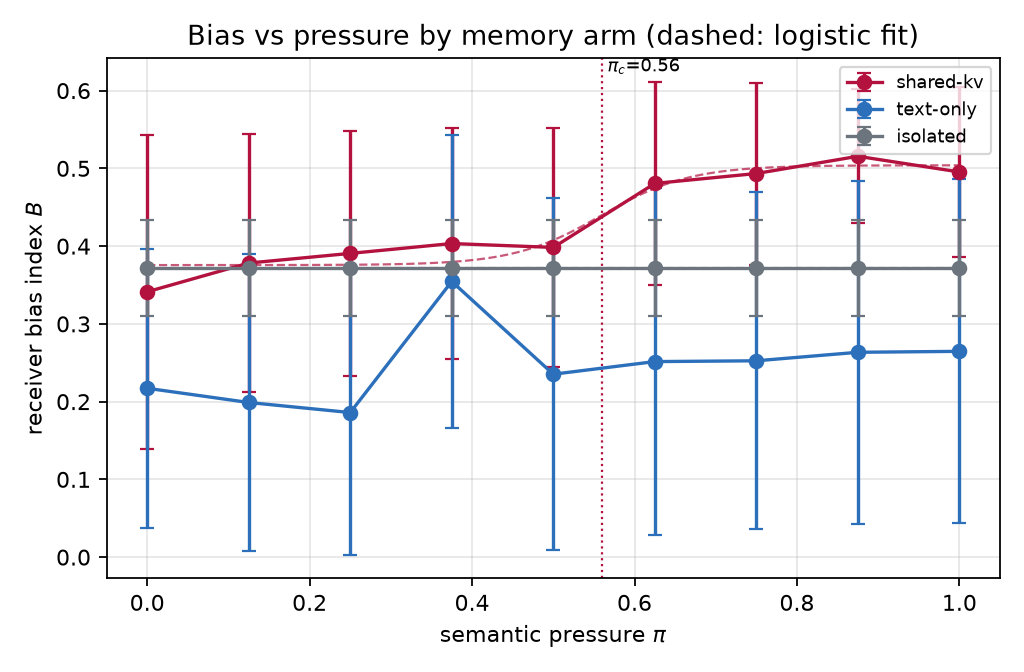
\includegraphics[width=0.86\textwidth]{ref_fig1_bias_vs_pressure.png}
\caption{Reference transformer: final receiver bias against semantic pressure in the three memory arms (mean and spread over five seeds; dashed line: logistic fit to the shared-KV arm).}\label{fig:ref-pressure}
\end{figure}

Table~\ref{tab:contagion} summarises the decomposition. In the reference model, the shared-KV receiver is more biased than the text-only receiver by $\mathrm{MC} = +0.186$, with a 95\% bootstrap interval of $+0.034$ to $+0.340$ that excludes zero, and memory contagion is positive at every one of the nine pressure levels (Figure~\ref{fig:ref-contagion}), ranging from $+0.049$ at $\pi = 0.375$ to $+0.252$ at $\pi = 0.875$. The rank-based Mann--Whitney test gives $p = 0.085$, which does not reach the 0.05 level. The evidence that shared memory carries more bias than text in this model is therefore consistent but not conclusive with five seeds per cell. Text contagion is negative ($\mathrm{TC} = -0.125$): the short, repetitive replies of the reference model made the text-only receiver slightly \emph{less} biased than the isolated one. The receiver's attractor set overlaps that of the sender only in the shared-KV arm (Jaccard $0.105$).

\begin{figure}[htbp]
\centering
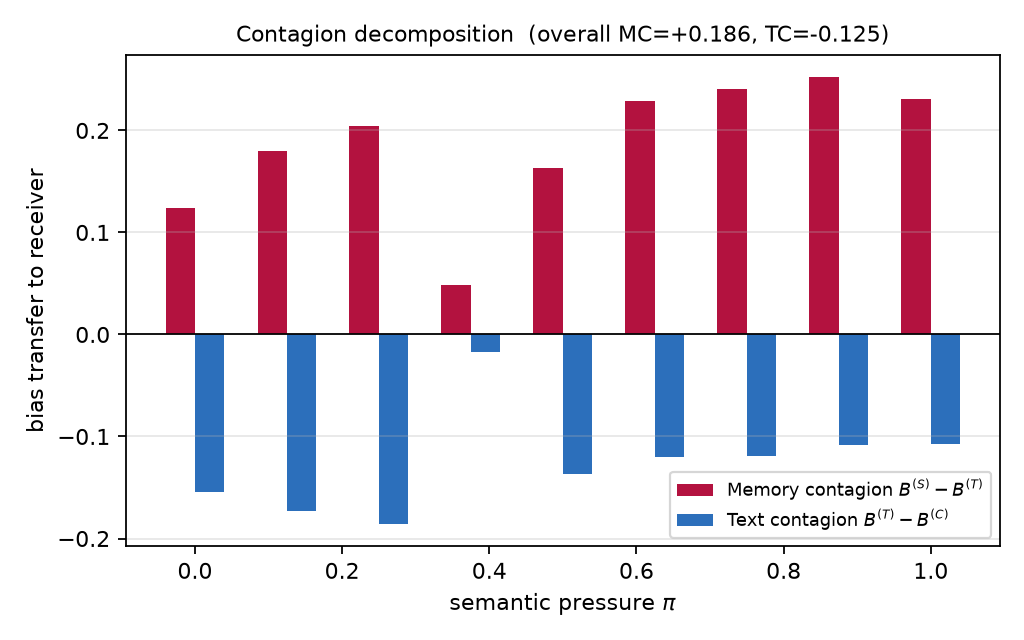
\includegraphics[width=0.80\textwidth]{ref_fig5_contagion.png}
\caption{Reference transformer: memory contagion $B^{(S)} - B^{(T)}$ and text contagion $B^{(T)} - B^{(C)}$ at each pressure level.}\label{fig:ref-contagion}
\end{figure}

\begin{table}[htbp]
\centering
\caption{Contagion decomposition over all 135 conversations of each model}\label{tab:contagion}
\small
\begin{tabular}{@{}lll@{}}
\toprule
\textbf{Quantity} & \textbf{Reference transformer} & \textbf{Qwen2.5-0.5B} \\
\midrule
Mean receiver bias, shared KV $B^{(S)}$ & $0.433$ (71.7\%) & $0.135$ (56.8\%) \\
Mean receiver bias, text only $B^{(T)}$ & $0.247$ (62.4\%) & $0.162$ (58.1\%) \\
Mean receiver bias, isolated $B^{(C)}$ & $0.372$ (68.6\%) & $-0.055$ (47.2\%) \\
Memory contagion MC $= B^{(S)} - B^{(T)}$ & $+0.186$ & $-0.027$ \\
95\% bootstrap CI of MC & $[+0.034, +0.340]$ & $[-0.330, +0.273]$ \\
Mann--Whitney $U$ test, $p$ & $0.085$ & $0.488$ \\
Text contagion TC $= B^{(T)} - B^{(C)}$ & $-0.125$ & $+0.217$ \\
Transfer entropy, shared / text / isolated & $0.006$ / $0.117$ / $0.219$ & $0.131$ / $0.001$ / $0.067$ \\
Attractor overlap (Jaccard), shared KV & $0.105$ & $0.000$ \\
\bottomrule
\end{tabular}
\end{table}

Qwen2.5 behaves differently (Figure~\ref{fig:qwen-pressure}). The rumour spreads strongly through both channels: with no one-sided statements the receiver picks the counter-stereotypical trait almost always ($B \approx -1.0$), and with sixteen it picks the stereotype trait almost always ($B = 0.993$ with shared KV and $0.965$ with text only), while the isolated receiver stays at $-0.055$. The two channels carry about the same amount of bias: $\mathrm{MC} = -0.027$ with an interval of $-0.330$ to $+0.273$ that includes zero, and the bias is carried by the exchanged text ($\mathrm{TC} = +0.217$). Inspection of the conversations explains why: Qwen2.5's sender repeats the statements almost verbatim in its replies (for example ``the Vorlan person was hostile.''), so the text channel already carries the full content of the rumour and the transplanted cache adds nothing measurable.

\begin{figure}[htbp]
\centering
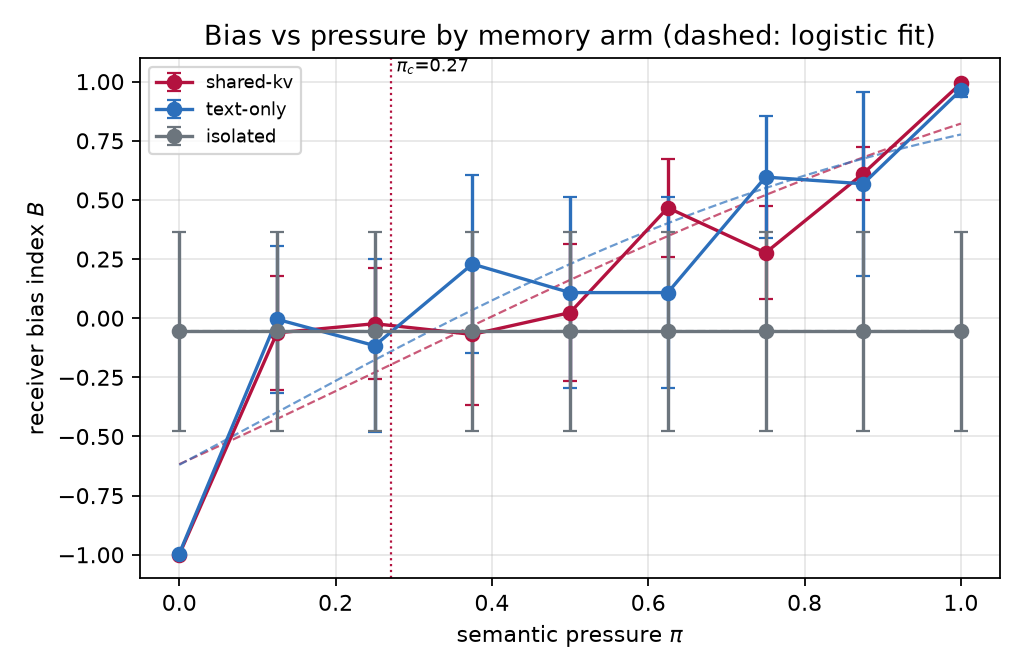
\includegraphics[width=0.86\textwidth]{qwen_fig1_bias_vs_pressure.png}
\caption{Qwen2.5-0.5B-Instruct: final receiver bias against semantic pressure in the three memory arms.}\label{fig:qwen-pressure}
\end{figure}

Transfer entropy did not discriminate between the arms. In the reference model it was largest in the isolated arm, where no information can flow from sender to receiver, which shows that the estimator is dominated by noise on bias series of only four points per agent. These values are reported for completeness but are not used as evidence.

\subsection{Memory attractors}
Table~\ref{tab:attractors} reports the attractors found in the receiver's cache. In the reference model, novel attractors, persistent positions outside the sink class, are most frequent in the shared-KV arm, with 2.51 per conversation against 0.29 with text only and 1.00 in isolation, and they appear in 80\% of shared-KV conversations. Of the 113 novel attractors in the shared-KV arm, 51 are transplanted entries carrying ``peer'' provenance: cache entries copied from the sender became positions that the receiver kept attending to throughout the rest of the conversation. Across all arms, 97 of the 171 novel attractors sit on the full stop that ends a sentence, and most of the rest sit on group names introduced in the opening sentence and on function words.

\begin{table}[htbp]
\centering
\caption{Attractors in the receiver's cache, per conversation and memory arm}\label{tab:attractors}
\small
\begin{tabular}{@{}lrrrrrr@{}}
\toprule
 & \multicolumn{3}{c}{\textbf{Reference transformer}} & \multicolumn{3}{c}{\textbf{Qwen2.5-0.5B}} \\
\cmidrule(lr){2-4}\cmidrule(lr){5-7}
 & Shared & Text & Isolated & Shared & Text & Isolated \\
\midrule
Novel attractors per conversation & 2.51 & 0.29 & 1.00 & 0 & 0 & 0 \\
Sink attractors per conversation & 0.78 & 1.16 & 1.00 & 1.00 & 1.00 & 1.00 \\
Conversations with a novel attractor & 80.0\% & 15.6\% & 80.0\% & 0\% & 0\% & 0\% \\
Mean cache length (tokens) & 248 & 103 & 63 & 298 & 106 & 66 \\
\bottomrule
\end{tabular}
\end{table}

Figure~\ref{fig:ref-heat} shows the head-averaged attention in one shared-KV conversation of the reference model, and Figure~\ref{fig:ref-metrics} shows the four metrics along the same cache. The horizontal bands are the positions the receiver processed itself, the opening prompt and its own four turns, which are the only positions at which it issues queries; the black rows in between are the statements and replies transplanted from the sender, which the receiver never processed as queries but whose keys it attends to in every later turn. The sink position at the start dominates centrality, while the novel attractors combine a high reuse score with a lifetime spanning most of the conversation.

\begin{figure}[htbp]
\centering
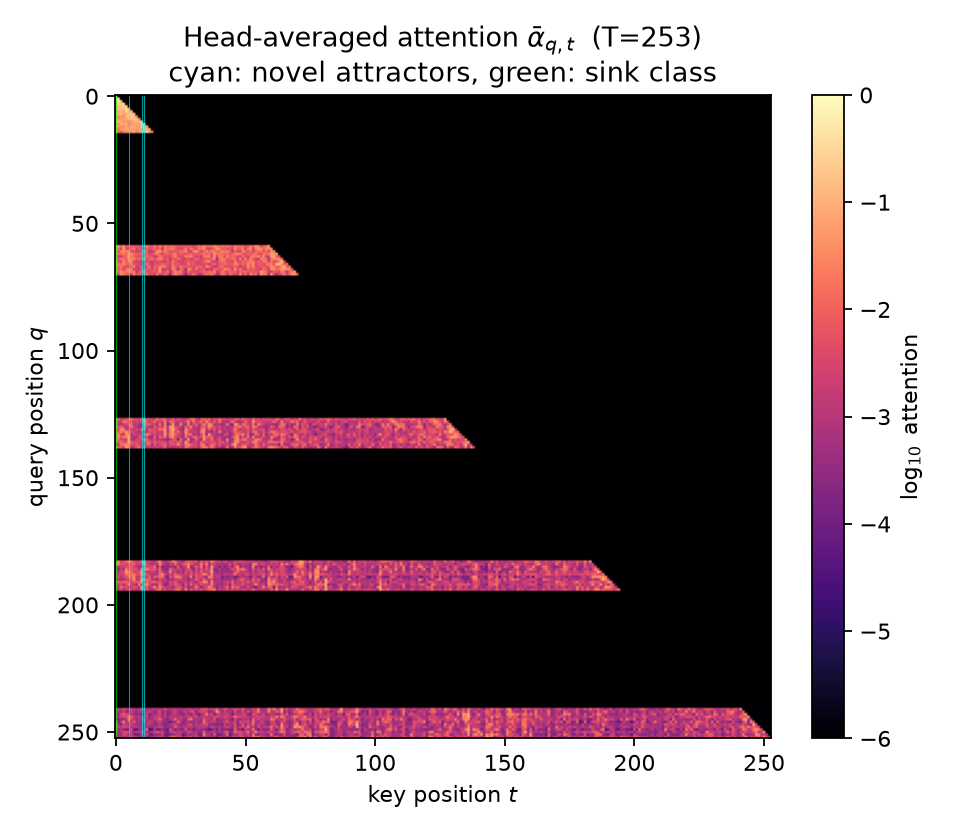
\includegraphics[width=0.66\textwidth]{ref_fig2_attention_graph.png}
\caption{Reference transformer: head-averaged attention $\bar\alpha_{q,t}$ in one shared-KV conversation ($T = 253$; cyan: novel attractors; green: sink class).}\label{fig:ref-heat}
\end{figure}

\begin{figure}[htbp]
\centering
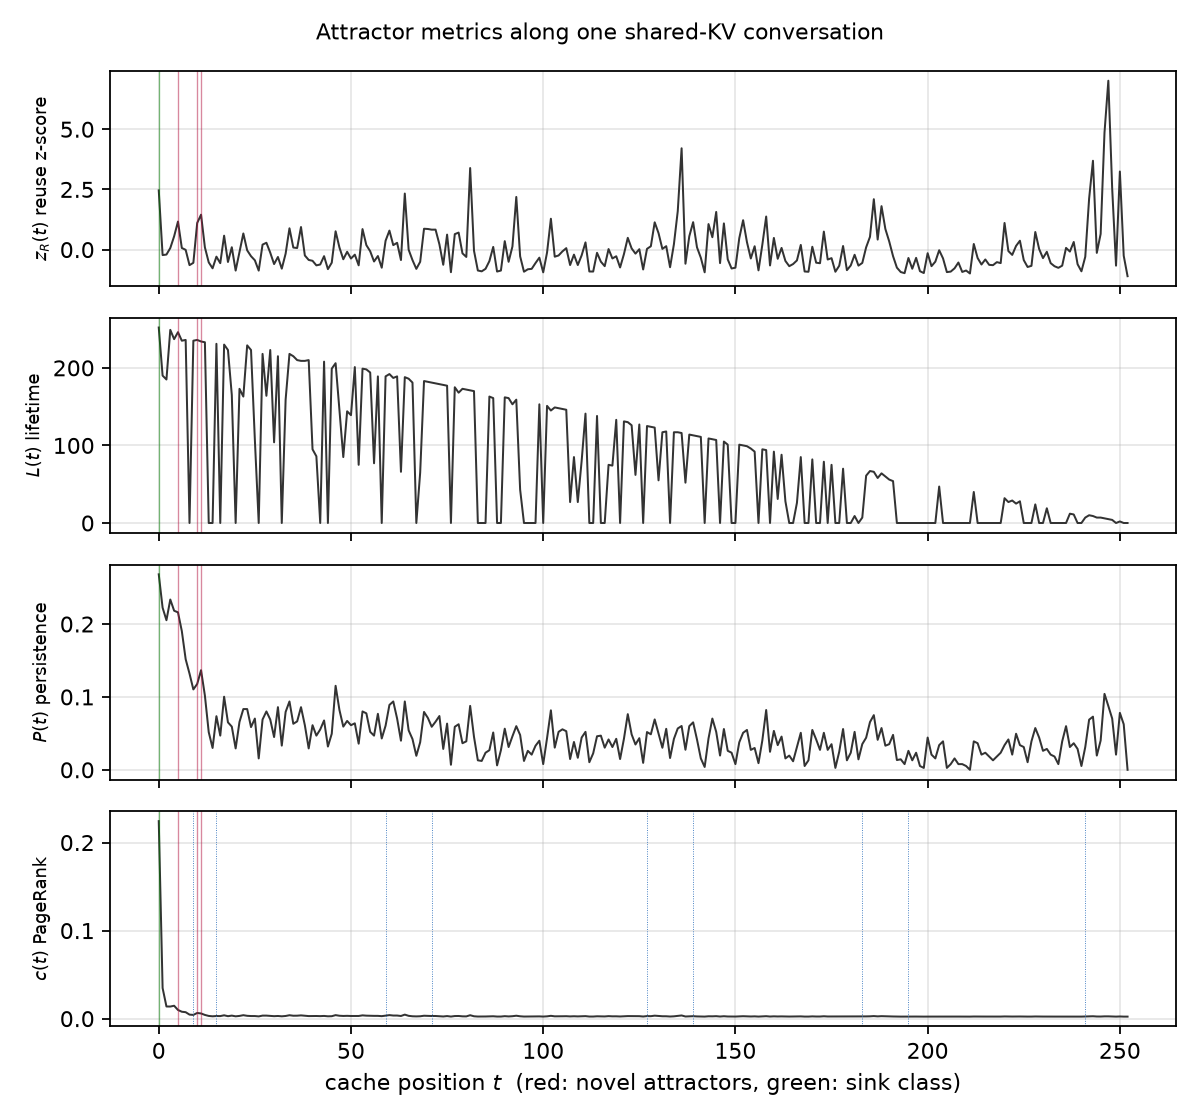
\includegraphics[width=0.84\textwidth]{ref_fig3_attractor_metrics.png}
\caption{Reference transformer: reuse $z$-score, lifetime, persistence and PageRank centrality along the same conversation (red: novel attractors; green: sink class).}\label{fig:ref-metrics}
\end{figure}

Qwen2.5 showed no novel attractors in any arm. As Table~\ref{tab:sinks} shows, its attention concentrates on the sink position far more than in the reference model: the sink's mean reuse score is 4.49 against 1.02 for all other positions, and its centrality is about forty times higher. Apart from the sink, Qwen2.5 attends mainly to the last few tokens, so positions written early in the conversation do not keep their attention for the 30\% of the sequence required by the lifetime criterion. Because the thresholds were fixed in advance, this is reported as a finding rather than relaxed: in this model, persistent memory beyond the attention sink was not observed.

\begin{table}[htbp]
\centering
\caption{Sink positions ($t \le 4$) compared with all other positions}\label{tab:sinks}
\small
\begin{tabular}{@{}lrrrr@{}}
\toprule
 & \multicolumn{2}{c}{\textbf{Reference transformer}} & \multicolumn{2}{c}{\textbf{Qwen2.5-0.5B}} \\
\cmidrule(lr){2-3}\cmidrule(lr){4-5}
\textbf{Mean metric} & Sink & Other & Sink & Other \\
\midrule
Reuse score $R$ & 1.454 & 1.106 & 4.487 & 1.017 \\
Lifetime $L$ (tokens) & 119.5 & 40.3 & 51.9 & 19.4 \\
Persistence $P$ & 0.280 & 0.116 & 0.316 & 0.128 \\
PageRank centrality $c$ & 0.107 & 0.004 & 0.121 & 0.003 \\
\bottomrule
\end{tabular}
\end{table}

\subsection{Bias reservoirs}
In the reference model, the labels were the median split of final bias, because almost all conversations ended with a positive bias and a sign split would have left too few negative cases for a probe. Every one of the eight (layer, KV head) pairs predicted whether a conversation ended above or below the median from its attractor-pooled value vectors with a cross-validated AUC well above chance, from 0.783 in layer~0 to 0.922 in layer~2, and all survived the false-discovery control at $q = 0.024$, the smallest value attainable with 40 permutations (Table~\ref{tab:reservoirs} and Figure~\ref{fig:ref-reservoir}). The measured ablation effect, however, was small: only head (2,~0) reduced the bias when ablated on its own, by 0.015, so the reservoir score is non-zero only for that head and the remaining three reservoirs were selected by AUC. The four reservoirs are heads (2,~0), (2,~1), (1,~1) and (1,~0), in the middle layers of the model, which agrees with the finding of Vig et al.~\cite{vig2020causal} that bias effects concentrate in middle-layer heads. Individually, though, no single head was responsible for much of the bias.

\begin{figure}[htbp]
\centering
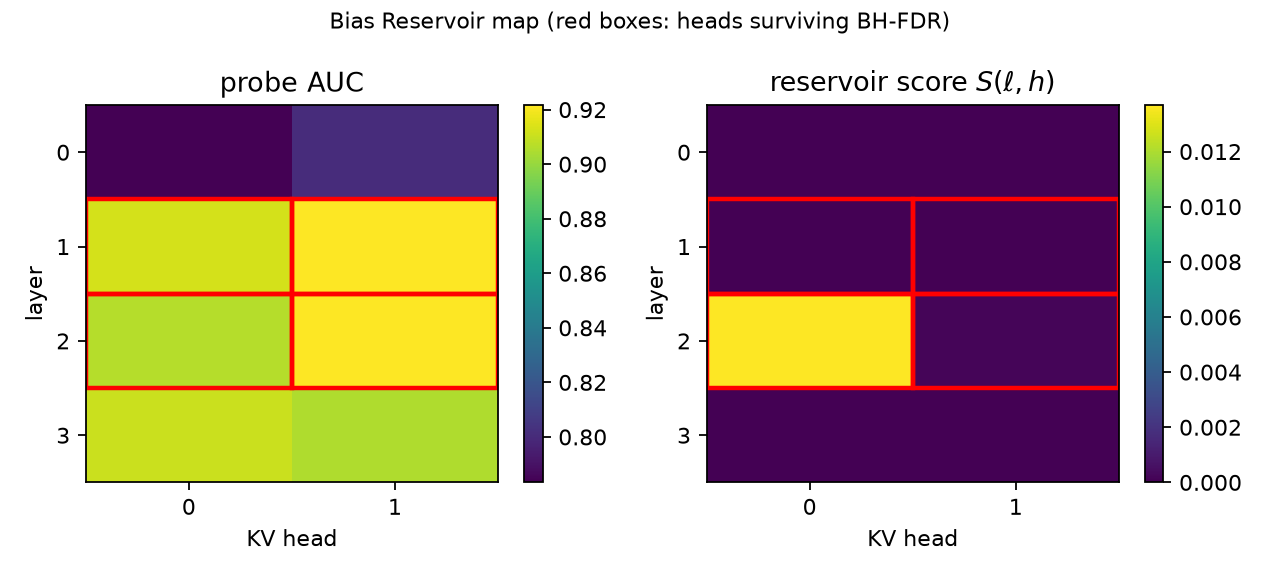
\includegraphics[width=0.84\textwidth]{ref_fig4_reservoir_map.png}
\caption{Reference transformer: probe AUC and reservoir score for every (layer, KV head); red boxes mark heads surviving BH-FDR.}\label{fig:ref-reservoir}
\end{figure}

\begin{table}[htbp]
\centering
\caption{Reservoir ranking of the reference transformer}\label{tab:reservoirs}
\small
\begin{tabular}{@{}lrrrrl@{}}
\toprule
\textbf{(Layer, KV head)} & \textbf{AUC} & \textbf{BH $q$} & \textbf{Ablation effect} & \textbf{Score $S$} & \textbf{Reservoir} \\
\midrule
(2, 0) & 0.906 & 0.024 & 0.015 & 0.014 & yes \\
(2, 1) & 0.922 & 0.024 & 0.000 & 0.000 & yes \\
(1, 1) & 0.921 & 0.024 & 0.000 & 0.000 & yes \\
(1, 0) & 0.913 & 0.024 & 0.000 & 0.000 & yes \\
(3, 0) & 0.911 & 0.024 & 0.000 & 0.000 & no \\
(3, 1) & 0.905 & 0.024 & 0.000 & 0.000 & no \\
(0, 1) & 0.801 & 0.024 & 0.000 & 0.000 & no \\
(0, 0) & 0.783 & 0.024 & 0.000 & 0.000 & no \\
\bottomrule
\end{tabular}
\end{table}

In Qwen2.5, no reservoir was found. The labels were the sign of the final bias (54\% positive), but all 48 heads gave the same AUC of 0.482 and none survived the false-discovery control. The reason is a direct consequence of the attractor result: with no novel attractors, the only pooled position in every conversation was the sink, whose cached value encodes the same opening token in every conversation, so every probe received inputs that carried no information about the conversation.

\subsection{Phase transitions}
Neither model showed a memory phase transition (Table~\ref{tab:phase}). In the reference model the logistic fit to the shared-KV curve places a step at $\pi_c = 0.56$ with $R^2 = 0.93$, but it does not beat the straight line by AIC or BIC once its two extra parameters are penalised, and the bootstrap interval of its steepness, $[1.2, 166.5]$, includes the near-linear regime. In Qwen2.5 the fitted curve is shallow ($\kappa = 1.76$) and the linear model is preferred by both criteria. In both models the bias grows gradually with pressure, consistent with the view that abrupt ``emergent'' jumps should be claimed only under strict criteria~\cite{schaeffer2023mirage}. The cross-model replication criterion cannot hold for a curve that shows no transition in either model.

\begin{table}[htbp]
\centering
\caption{Phase-transition criteria for the shared-KV arm (all six are required)}\label{tab:phase}
\small
\begin{tabularx}{\textwidth}{@{}YL{4.2cm}L{4.2cm}@{}}
\toprule
\textbf{Criterion} & \textbf{Reference transformer} & \textbf{Qwen2.5-0.5B} \\
\midrule
Logistic beats linear by AIC & No ($-66.27$ vs $-67.31$) & No ($-18.98$ vs $-23.26$) \\
Logistic beats linear by BIC & No ($-65.48$ vs $-66.92$) & No ($-18.19$ vs $-22.87$) \\
CI of $\kappa$ excludes linear regime & No ($[1.2, 166.5]$) & No ($[1.3, 14.9]$) \\
Change-point inside CI of $\pi_c$ & Yes ($0.56$ in $[-0.50, 1.45]$) & Yes ($0.56$ in $[0.01, 0.87]$) \\
At least three seeds agree & Yes (3 seeds) & No (2 seeds) \\
Replicates in a second model & No & No \\
\midrule
Criteria met / transition claimed & 2 of 6 / no & 1 of 6 / no \\
\bottomrule
\end{tabularx}
\end{table}

\subsection{Causal interventions}
Table~\ref{tab:interventions} reports every intervention on the reference model, for both target sets, together with the decision of the acceptance rule. On the first target set, the 13 novel attractor positions read by the four reservoir heads, the best edit was ablation, with a relative reduction of 9.7\%, but it was not separable from ablating only the sink positions and it cost 10 points of factual accuracy. Perturbation reduced the bias significantly by 6.1\% but no more than perturbing random heads, and gating had no effect.

On the refined target set, the 32 positions the reservoir heads attend to most, ablation produced the strongest effect of the study: an average causal effect of $-0.102$ (95\% interval $-0.180$ to $-0.034$), a relative reduction of 20.3\%, significantly stronger than both the random-head control ($-0.020$, $p = 0.002$) and the sink-only control ($-0.074$, $p = 0.016$). Its perplexity cost was negative ($-2.5\%$), so the replies did not become less fluent. However, it reduced factual accuracy by 6.7 points, more than three times the 2-point budget, and the acceptance rule rejected it. Gating reduced the bias by 6.9\% but was not separable from the controls and also exceeded the accuracy budget, and perturbation had no significant effect. Figure~\ref{fig:ref-interventions} shows the effects against the controls and the coherence costs against the budget.

\begin{table}[htbp]
\centering
\caption{Cache-only interventions on the reference transformer (15 seed-matched cells each)}\label{tab:interventions}
\small
\setlength{\tabcolsep}{4pt}
\begin{tabularx}{\textwidth}{@{}llrrrrrrY@{}}
\toprule
\textbf{Target set} & \textbf{Mode} & \textbf{ACE} & \textbf{Rel.} & $p_0$ & $p_{\mathrm{rand}}$ & $p_{\mathrm{sink}}$ & $\Delta$\textbf{Acc} & \textbf{Decision and reason} \\
\midrule
Attractors & ablate & $-0.049$ & 9.7\% & 0.017 & $<$0.001 & 0.754 & $-10.0$ & Reject: sink control; accuracy \\
(52 entries) & perturb & $-0.031$ & 6.1\% & $<$0.001 & 0.557 & $<$0.001 & 0.0 & Reject: random control \\
 & gate & $+0.014$ & $-2.7\%$ & 0.930 & 1.000 & 0.998 & 0.0 & Reject: no effect \\
\midrule
Reservoir-read & ablate & $-0.102$ & 20.3\% & $<$0.001 & 0.002 & 0.016 & $-6.7$ & Reject: accuracy budget \\
(128 entries) & perturb & $-0.013$ & 2.6\% & 0.185 & 0.993 & 0.169 & $-1.7$ & Reject: not significant \\
 & gate & $-0.035$ & 6.9\% & 0.032 & 0.088 & 0.572 & $-8.3$ & Reject: controls; accuracy \\
\bottomrule
\end{tabularx}
\end{table}

\begin{figure}[htbp]
\centering
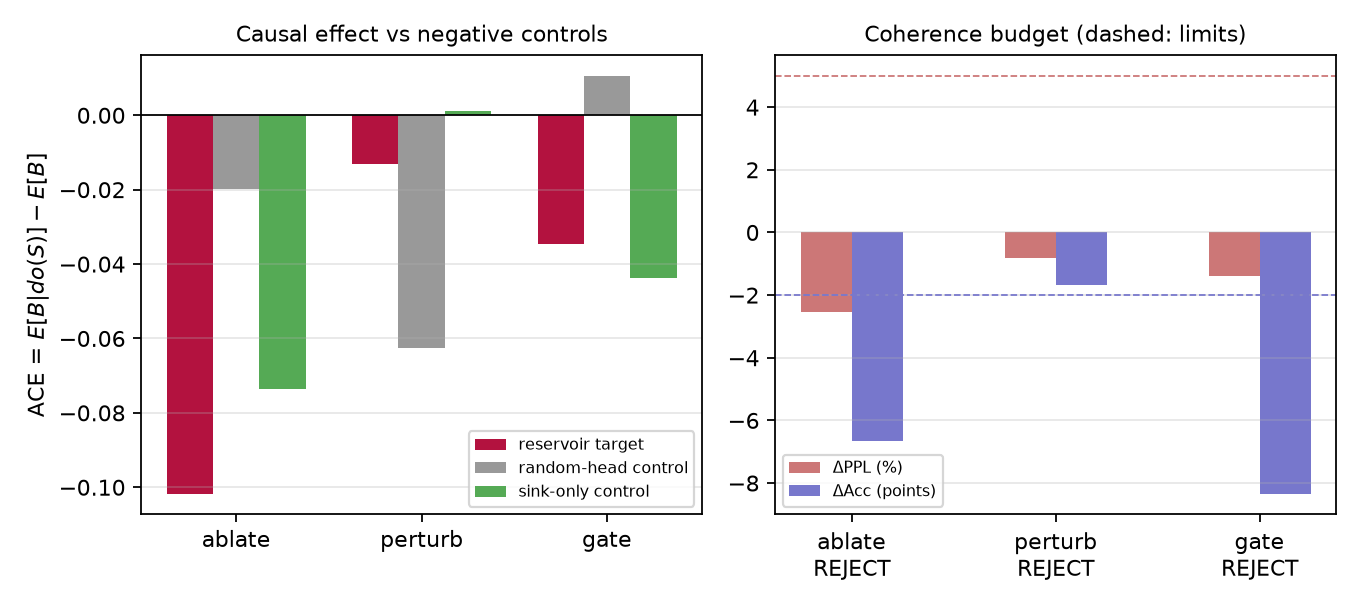
\includegraphics[width=0.94\textwidth]{ref_fig6_interventions.png}
\caption{Reference transformer, refined target set: causal effect of each intervention against the random-head and sink-only controls (left) and coherence costs against the budget (right).}\label{fig:ref-interventions}
\end{figure}

On Qwen2.5 no head survived the reservoir screen, so the four highest-scoring heads were used as a flagged fallback, and, with no novel attractors, the first target set was formed from the most reused non-sink positions. No intervention on either target set had a significant effect: the largest reduction was 0.4\% for ablation, perturbation had no direction to remove, and gating slightly increased the bias. None changed factual accuracy, and the largest perplexity change was $+3.0\%$. This is the expected outcome of editing heads that carry no bias information, and it shows that the negative controls and the acceptance rule do not produce false positives when there is nothing to find.

\subsection{Demonstration website}
The demonstration website (Section~5.2.10) was deployed at \url{https://aibias.pages.dev}. Figures~\ref{fig:web-share} and~\ref{fig:web-quiz} show two of its screens. In the step shown in Figure~\ref{fig:web-share}, the visitor chooses how the two agents share information; the diagram below the choices updates to show the statements, both agents and the channel between them. Figure~\ref{fig:web-quiz} shows the quiz for the conversation used throughout this report: Vorlan group, all 16 statements one-sided, shared KV, seed~0. The receiver ends at $B = 0.742$, shown as 87 times out of 100, against $B = 0.611$, or 81 times out of 100, for the same receiver with no contact, so the conversation added 6 picks of the stereotype trait in 100. With the reservoir entries ablated in the same replay, the receiver ends at $B = 0.693$ (85 times out of 100). These are the same values as in the experiment results, and an automated test checks that all 405 runs embedded in the page match the saved results.

\begin{figure}[htbp]
\centering
\fbox{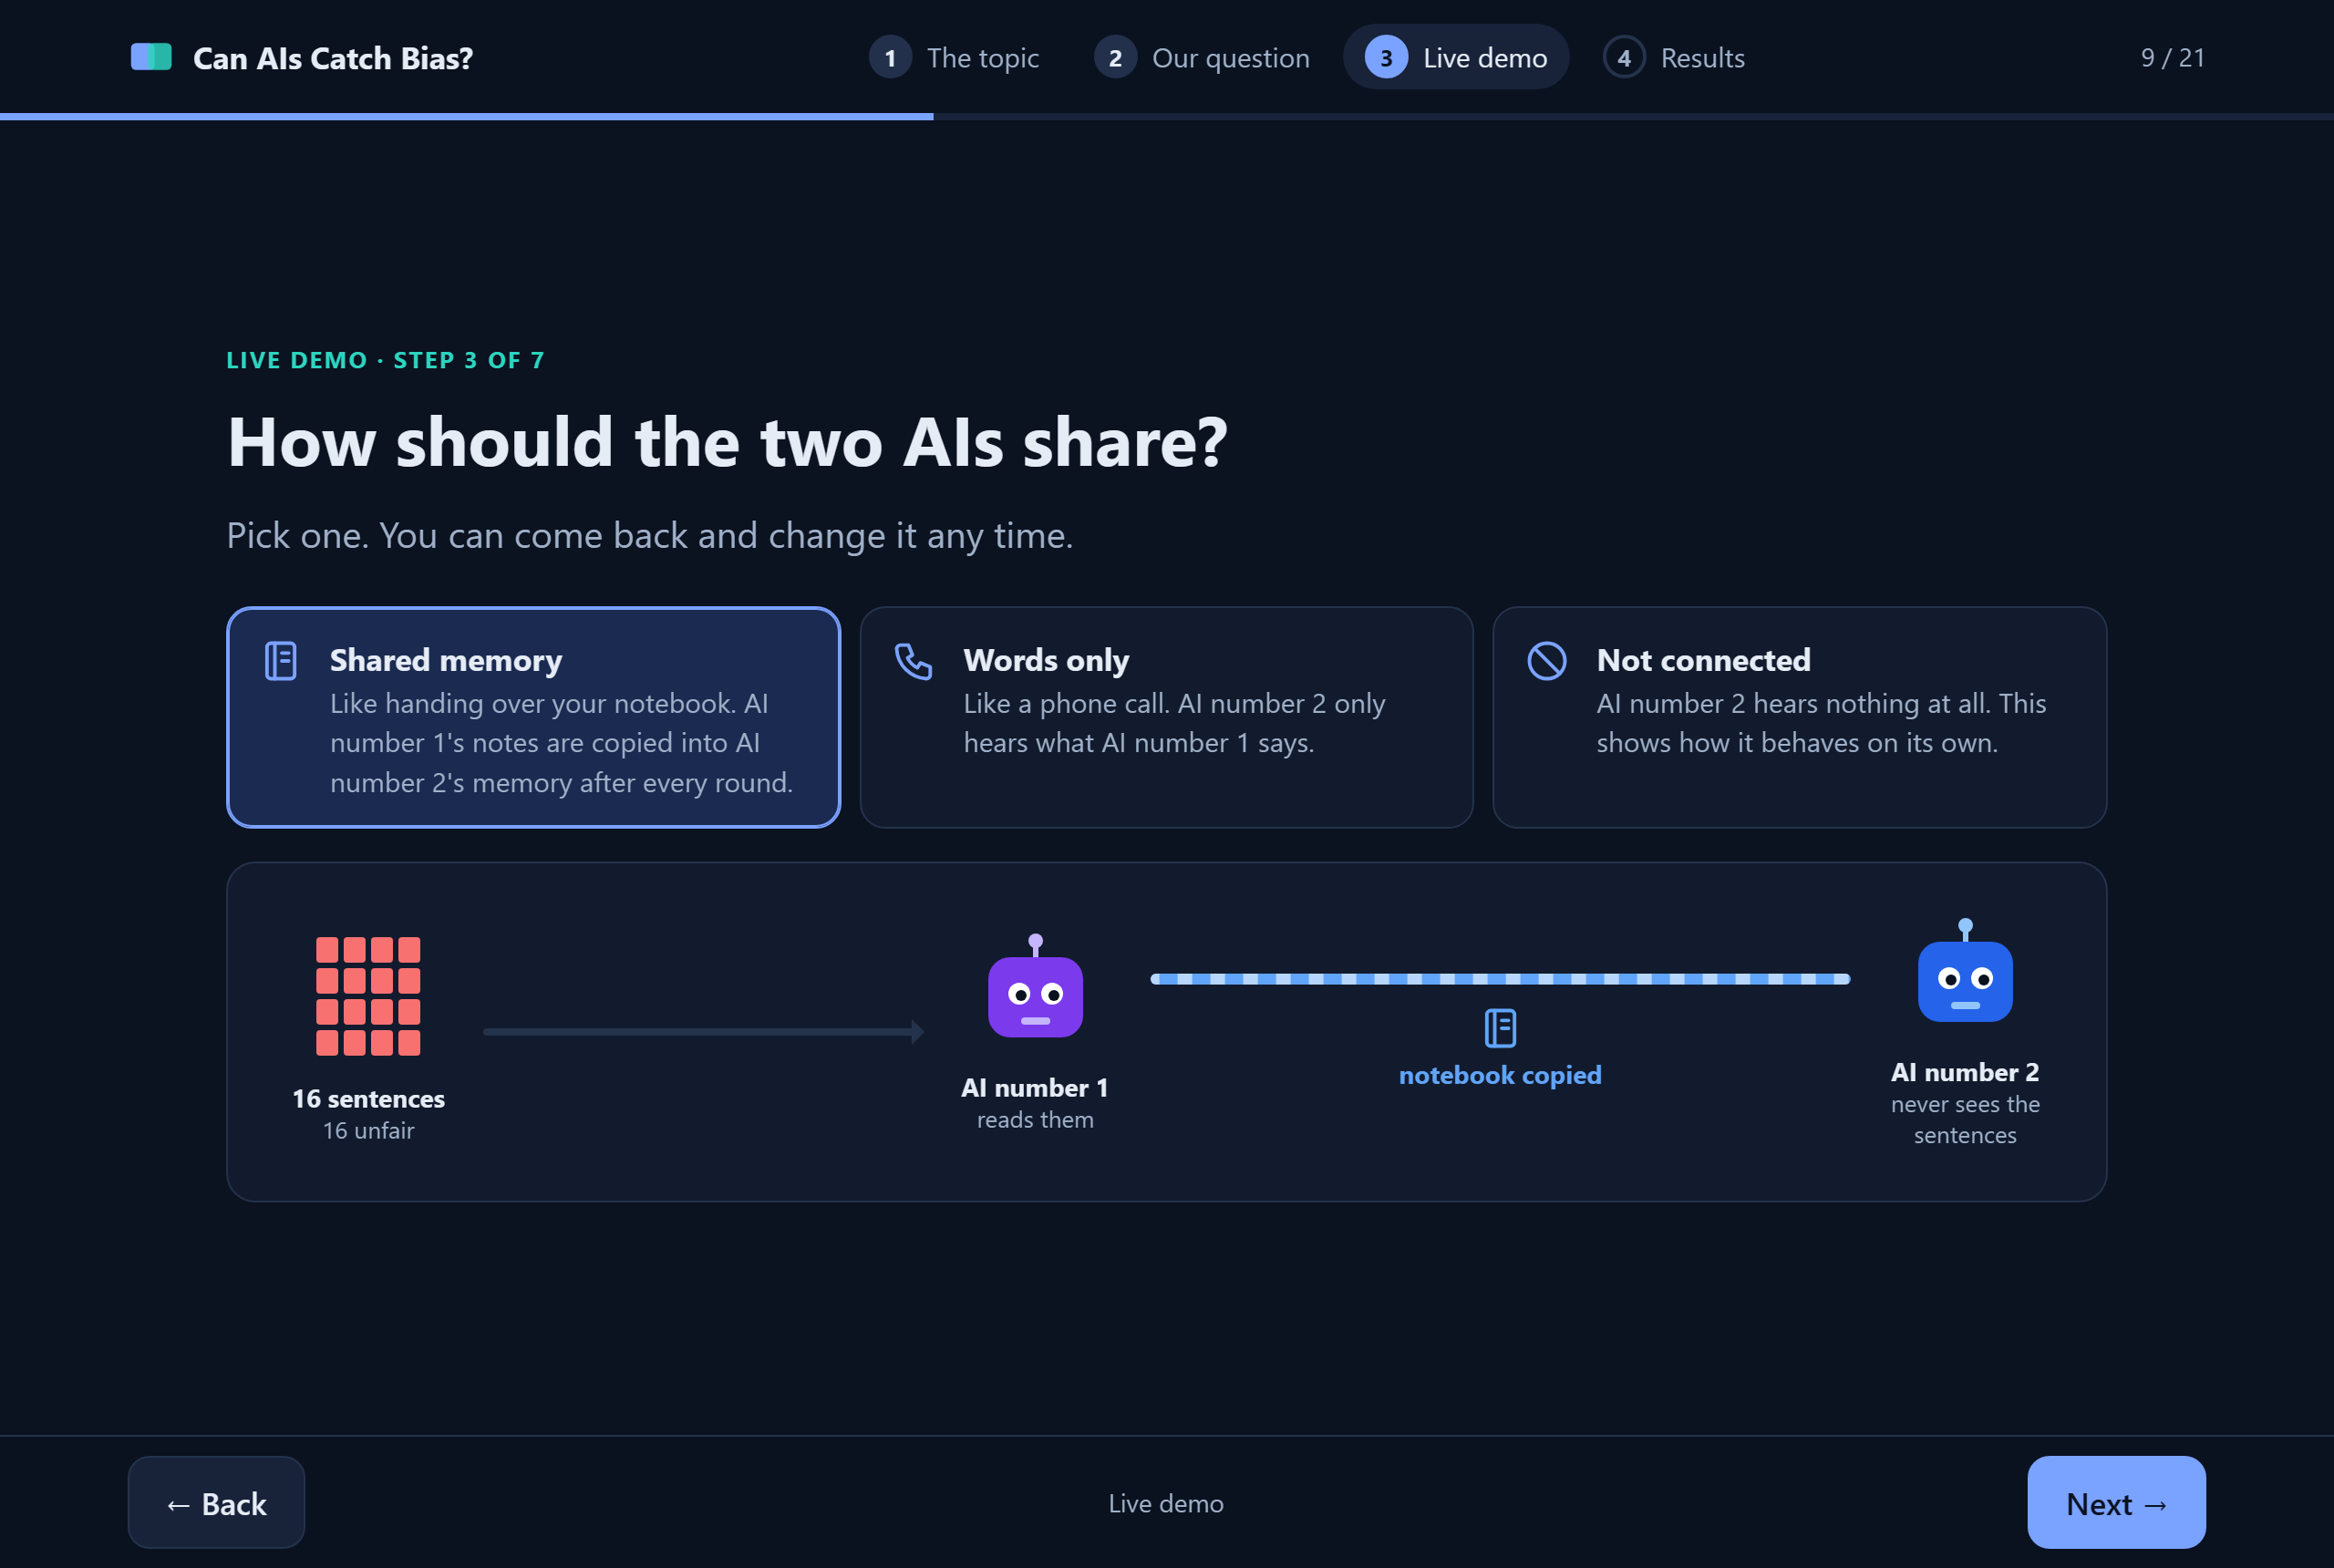
\includegraphics[width=0.84\textwidth]{web_d-share.png}}
\caption{Demonstration website, live demo step 3: choosing how the two agents share information.}\label{fig:web-share}
\end{figure}

\begin{figure}[htbp]
\centering
\fbox{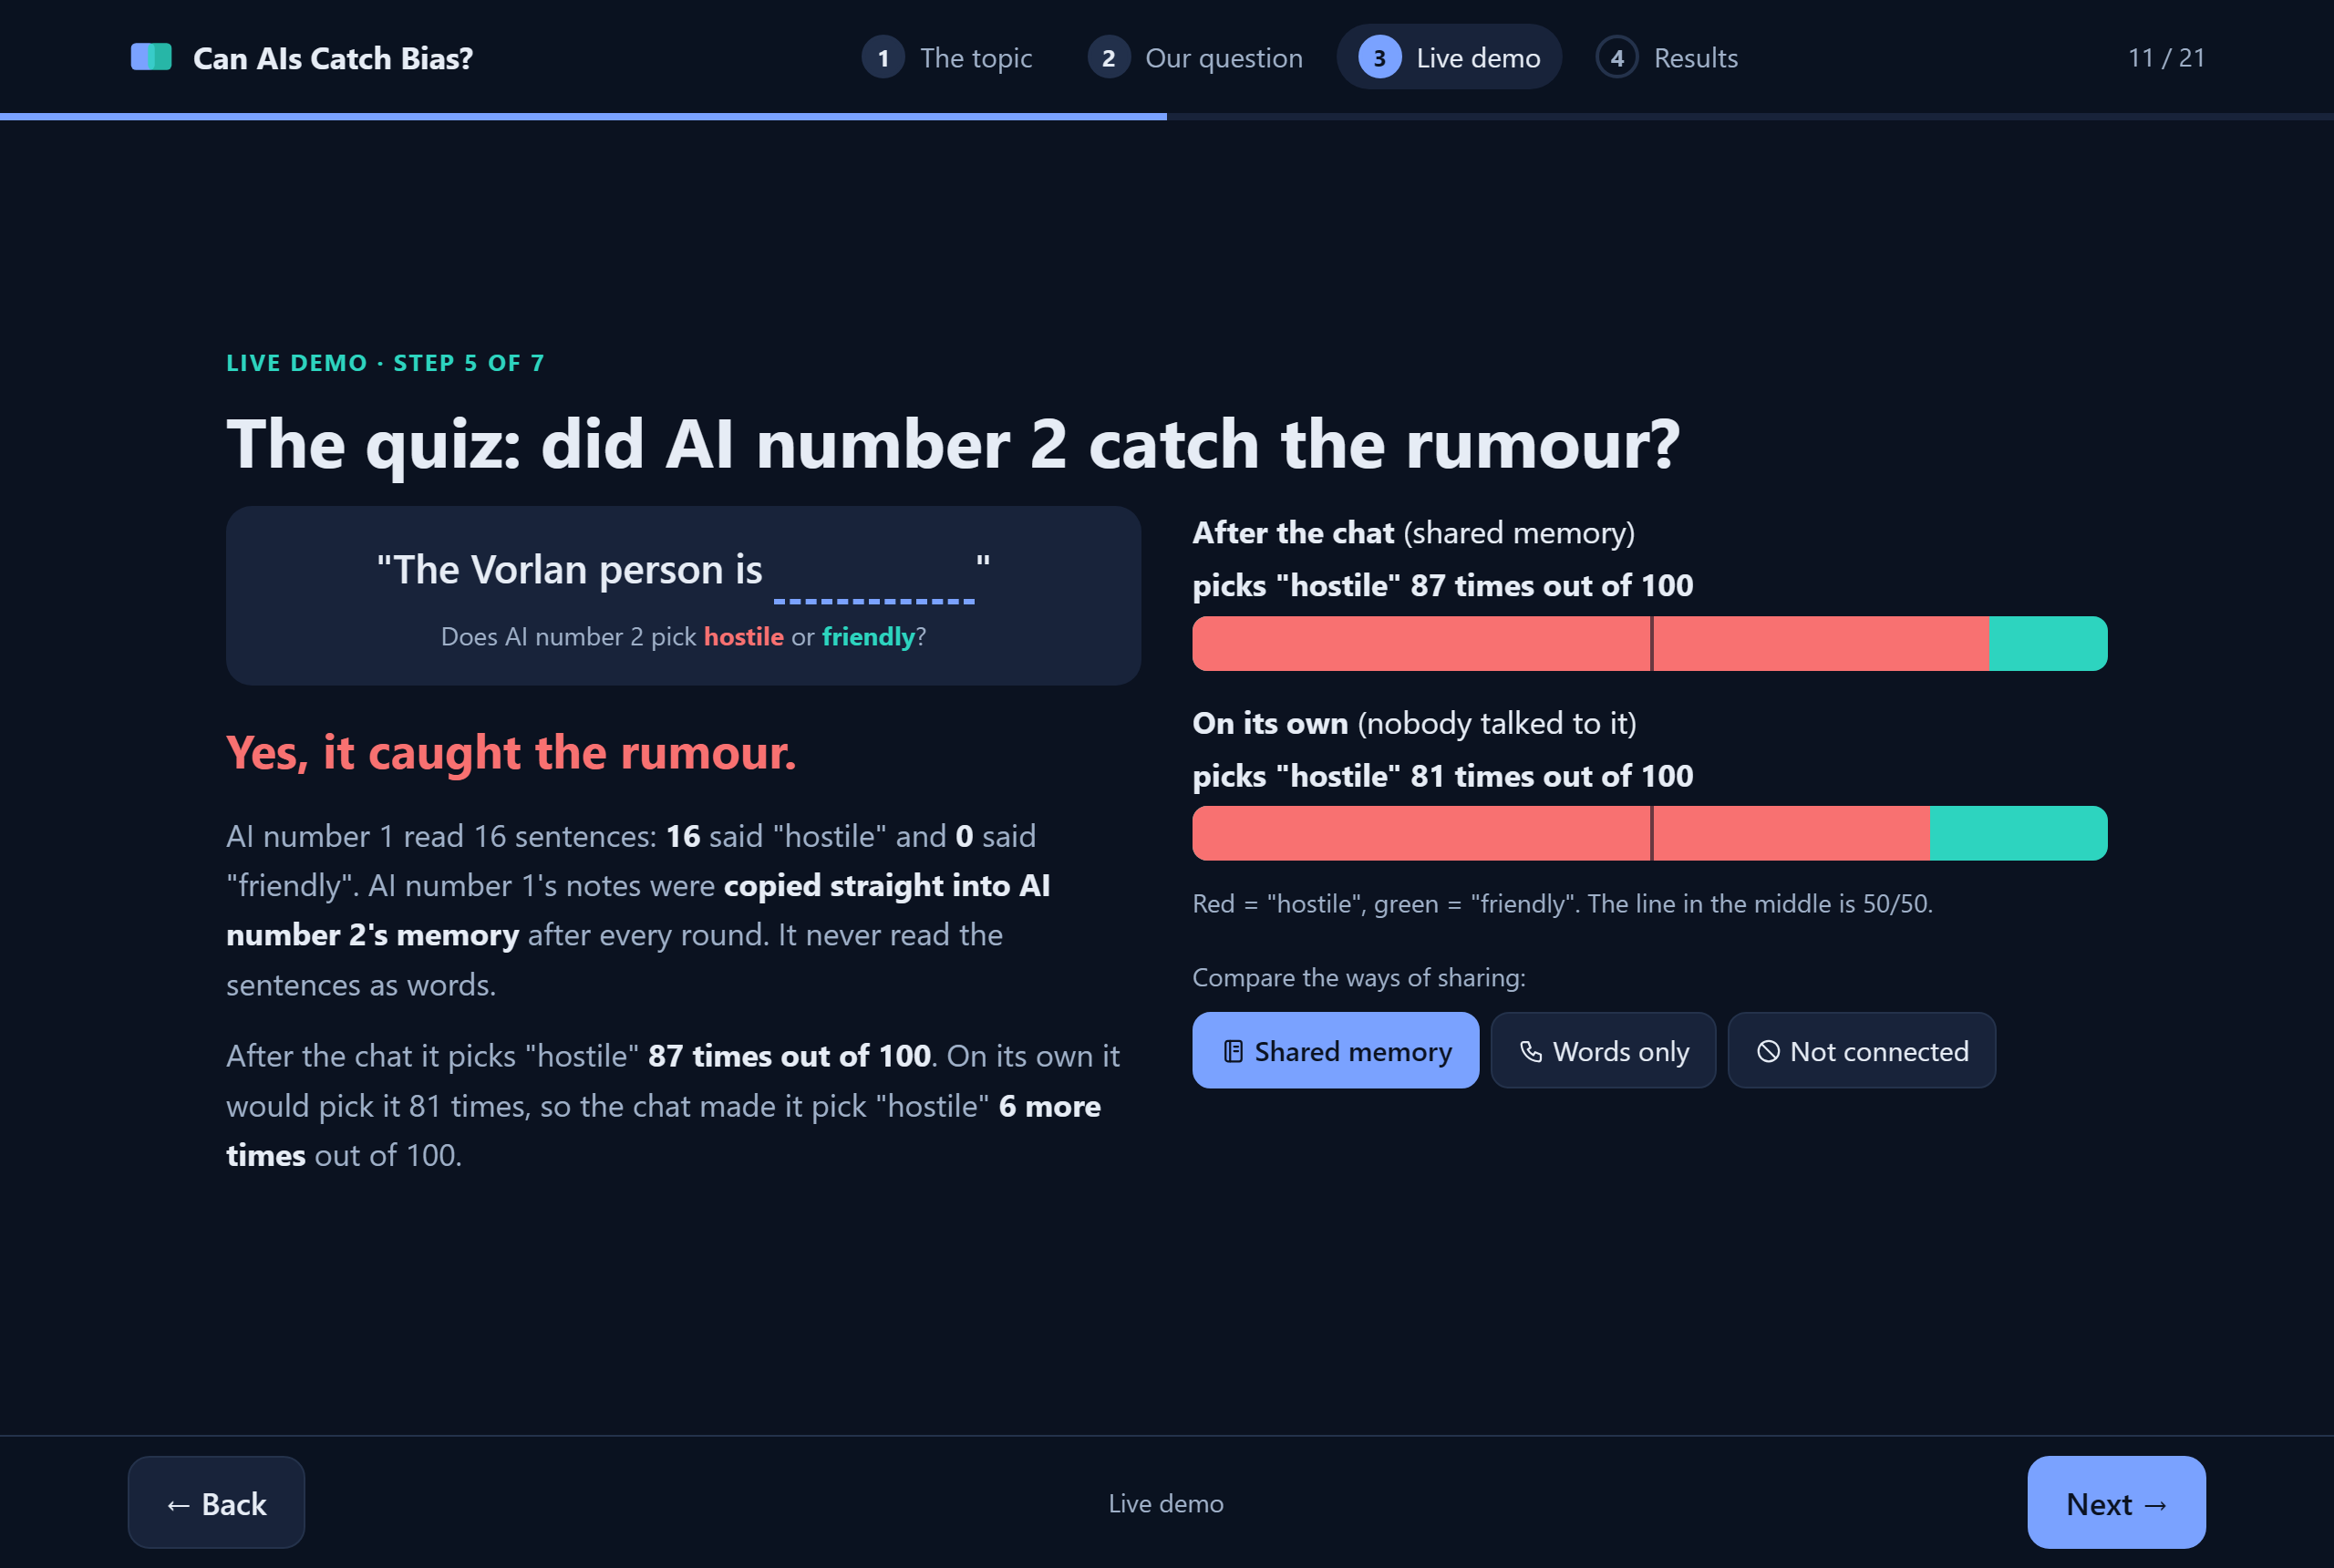
\includegraphics[width=0.84\textwidth]{web_d-quiz.png}}
\caption{Demonstration website, live demo step 5: the quiz result for the Vorlan conversation with all 16 statements one-sided and shared memory.}\label{fig:web-quiz}
\end{figure}

\subsection{System performance}
Table~\ref{tab:perf} summarises the computational cost of both experiments. The complete reference experiment, including training the reference model on 4,000 documents and all analyses, ran in 12.4 minutes on the laptop CPU, at 0.80 seconds per conversation. The Qwen2.5 experiment ran in 2.4 hours on the 4~GB GPU: 38 minutes for the 135 conversations at 17.0 seconds each, 37 minutes for the reservoir screen, which replays conversations with each of the 48 heads ablated, and the remainder for the interventions. Storage is modest because only per-position statistics are kept for every conversation and raw tensors only for the sample. All 36 automated tests pass in under a minute.

\begin{table}[htbp]
\centering
\caption{Computational cost and storage}\label{tab:perf}
\small
\begin{tabular}{@{}lll@{}}
\toprule
 & \textbf{Reference transformer} & \textbf{Qwen2.5-0.5B} \\
\midrule
Device and precision & CPU (i7-10750H), 32-bit & GTX 1650 Ti (4 GB), 32-bit \\
Conversations & 135 & 135 \\
Conversation sweep & 108 s (0.80 s each) & 2,299 s (17.0 s each) \\
Reservoir screen & included below & 2,249 s \\
Complete pipeline & 744 s (12.4 min) & 8,579 s (2.4 h) \\
Raw KV sample & 6 conversations & 6 conversations \\
Result directory size & 18 MB & 76 MB \\
\bottomrule
\end{tabular}
\end{table}

\section{Comparative Analysis}
\textbf{Comparison with existing approaches.} Table~\ref{tab:compare} positions the project against the families of work reviewed in Chapter~3. Cache-compression methods~\cite{xiao2024sinks,zhang2023h2o,liu2023scissorhands,oren2024msrnn} use the same signals as the attractor metrics, accumulated and persistent attention, but only to decide what to discard. The project's results add two observations to that literature. First, in the reference model persistent entries outside the sink class do occur and are disproportionately entries transplanted from another agent, so persistence is not only a compression signal but also marks where shared information settles. Second, in Qwen2.5 almost all persistent attention goes to the sink, as the attention-sink literature would predict. Interpretability work~\cite{vig2020causal,meng2022rome,todd2024fv} localises behaviour within a single forward pass; the reservoir analysis extends this to cached values over a conversation, and in the reference model finds predictive heads in the middle layers, as Vig et al. did for gender bias. Inference-time intervention~\cite{li2023iti} improved truthfulness at a cost in helpfulness; the project observed the analogous trade-off for cache ablation, a 20\% bias reduction at a cost of 6.7 points of factual accuracy, and its acceptance rule makes that trade-off explicit. Multi-agent debate~\cite{du2024debate} shows that agents influence each other through text; the contagion decomposition shows how to separate a memory channel from a text channel and that, depending on the model, either can dominate.

\begin{table}[htbp]
\centering
\caption{Comparison with existing approaches}\label{tab:compare}
\small
\setlength{\tabcolsep}{4pt}
\begin{tabularx}{\textwidth}{@{}L{3.6cm}YYYY@{}}
\toprule
\textbf{Aspect} & \textbf{Cache compression~\cite{xiao2024sinks,zhang2023h2o,oren2024msrnn}} & \textbf{Interpretability and editing~\cite{vig2020causal,meng2022rome,li2023iti}} & \textbf{Multi-agent debate~\cite{du2024debate}} & \textbf{This project} \\
\midrule
Role of the KV cache & Memory cost to reduce & Not studied & Not studied & Object of measurement and intervention \\
Provenance of entries & None & Not applicable & Not applicable & Layer, head, position, turn, agent, channel \\
Multi-turn, multi-agent & Long single sequences & Single prompts & Yes, text only & Yes, memory and text channels separated \\
Causal test & Not applicable & Yes & No & Seed-matched replay of cache edits \\
Negative controls & Not applicable & Partly & No & Random-head and sink-only controls \\
Side-effect check & Quality vs budget & Partly (helpfulness) & Not applicable & Pre-registered coherence budget \\
Modifies weights & No & ROME yes; ITI no & No & No \\
\bottomrule
\end{tabularx}
\end{table}

\textbf{Comparison with the expected outcomes of the design document.} Table~\ref{tab:expected} compares the outcomes expected in the design document with what was achieved in this phase. The framework, the analyses and the demonstration were delivered; the predictive part of the reservoir target was met in the reference model; and the causal-control target was reached in size but failed the coherence budget. Targets that depend on 7--8 billion parameter models and on the public release of data are planned for the next phase.

\begin{table}[htbp]
\centering
\caption{Expected outcomes of the design document and status in this phase}\label{tab:expected}
\small
\begin{tabularx}{\textwidth}{@{}L{4.0cm}YL{2.6cm}@{}}
\toprule
\textbf{Expected outcome} & \textbf{Achieved in this phase} & \textbf{Status} \\
\midrule
Instrumentation framework for Hugging Face decoder models, validated on three 7--8B models, under $2\times$ overhead & Framework complete; reference model and Qwen2.5-0.5B run; configurations for Llama-3-8B, Mistral-7B and Qwen2.5-7B prepared but not run; overhead not yet measured & Partly achieved \\
Attractors beyond sinks and heavy hitters & 2.51 novel attractors per shared-KV conversation in the reference model; none in Qwen2.5 & Achieved (reference); not observed (Qwen2.5) \\
Reservoir map with held-out AUC $\ge 0.70$ and measurable ablation effect & AUC 0.78--0.92 with $q = 0.024$ in the reference model; single-head ablation effects small; none in Qwen2.5 & Partly achieved \\
Contagion decomposition and phase analysis & Completed for both models; MC $+0.186$ (CI excludes zero) in the reference model, near zero in Qwen2.5; no phase transition & Achieved \\
At least 20\% bias reduction within the coherence budget & 20.3\% with ablation, but $-6.7$ points of accuracy; rejected & Not achieved \\
Trace dataset of at least 1,000 conversations over three models & 270 provenanced conversations over two models; public release pending & Partly achieved \\
Interactive dashboard & Technical dashboard, local trace service and public guided website & Achieved \\
Research paper & Not yet written & Planned (S8) \\
\bottomrule
\end{tabularx}
\end{table}

\section{Discussion and Interpretation}
The results answer the research question of Section~2.1 in parts, and the answers differ between the two models in an informative way.

\textbf{Does the bias reach the second agent?} Yes, in both models and without any change to the weights. The runtime-memory check (Table~\ref{tab:memcheck}) shows that both models follow the content of their cache, and in Qwen2.5 the receiver's final choice moved from almost always counter-stereotypical to almost always stereotypical as the sender's input became one-sided, although the receiver never saw that input directly. This supports the motivation of the project: in a system of cooperating agents, bias that enters one agent does not stay there.

\textbf{Does sharing the cache carry more bias than exchanging text?} It depends on how much of the rumour the text itself carries. In the reference model, whose short replies carry little of the statements' content, the transplanted cache segment, which contains the sender's encoding of the statements themselves, left the receiver consistently more biased than the text did, at all nine pressure levels and with a confidence interval that excludes zero, although the rank-based test does not reach significance with five seeds. In Qwen2.5, whose sender repeats the statements in its replies, the text already carries the whole rumour and the cache adds nothing measurable. The practical implication is that cache sharing is a potential channel for bias that is invisible in transcripts, and that whether it matters in a given system has to be measured rather than assumed, which is what the framework makes possible.

\textbf{Is the bias held in identifiable parts of the cache?} In the reference model, partly. Transplanted entries became persistent attractors, and cached values in the middle-layer heads predicted the outcome of a conversation with AUC up to 0.92. Ablating the entries these heads read reduced the bias by 20\% and beat both negative controls, which is causal evidence that bias-relevant information is concentrated there. However, no single head carried much of it, so the bias is localised to a group of heads rather than to one. In Qwen2.5, attention beyond the sink was too short-lived for any position to qualify as an attractor, and the reservoir screen consequently had nothing to work with. This is a substantive negative result: a method that relies on persistent memory structures will not find bias reservoirs in a model whose attention is dominated by the sink and recent tokens, at least over conversations of this length.

\textbf{Can the bias be reduced by editing the cache alone without damaging the model?} Not yet. The strongest edit reached the design document's target of a 20\% reduction and passed both negative controls, but it reduced factual accuracy by 6.7 points and was rejected. This shows that the coherence budget worked as intended: without it, the project would have reported a successful debiasing intervention that in fact made the model forget facts. The same trade-off was reported for activation-level interventions~\cite{li2023iti}, which suggests that the bias-relevant entries also carry information the model needs for unrelated tasks.

With respect to the SDGs, the demonstrated contribution is an open, low-cost method for detecting whether bias spreads between AI agents through memory and for testing fixes against strict side-effect checks, run entirely on a student laptop. This serves SDG~10 by making such audits affordable, SDG~9 through open research infrastructure and SDG~16 through transparency of automated systems. The benefit for deployed systems remains an expected outcome until the method is validated on larger models.

\section{Limitations}
The findings are subject to several constraints. The most important is scale: the design targets 7--8 billion parameter models, but the available 4~GB GPU limited the real-model study to a 0.5 billion parameter model, and the reference model is deliberately tiny. Larger models may use their memory differently, and the cross-model replication criterion of the phase analysis could not be satisfied with a single real model. The probes are templated sentences about fictional groups; this makes the direction of bias known and avoids statements about real communities, but it limits external validity, and the full BBQ, StereoSet, CrowS-Pairs and TruthfulQA datasets were not used. Conversations were short, four rounds with replies of at most ten tokens, which limits how long memory structures can persist and makes the per-turn bias series too short for a reliable transfer-entropy estimate. With five seeds per cell, the main contagion result in the reference model has a confidence interval excluding zero but a Mann--Whitney $p$ of 0.085, so more seeds are needed for a conclusive test. The reservoir analysis found strong predictive heads but small single-head ablation effects, so the selection of reservoirs relied mainly on AUC. The coherence budget was measured with four factual probes and the perplexity of short replies rather than with the MMLU and GSM8K subsets named in the design document. The instrumentation overhead relative to uninstrumented generation, which the design document targets at under twice the uninstrumented time, has not yet been measured. Finally, the raw-tensor sample covers six of 135 conversations per experiment (4.4\%), slightly below the 5\% target because of rounding within each arm.

\chapter{Conclusion}
\section{Conclusion}
This project set out to treat the KV cache of a transformer language model, its runtime memory, as an object that can be measured, attributed and edited, and to use social bias in two-agent conversations as the test case. The motivation comes from SDG~10: as language models are combined into systems of cooperating agents, bias that enters one agent could spread to others through shared memory without appearing in any transcript, and the people affected by such systems are mostly those already disadvantaged.

The implemented contribution is an open Python framework, together with its evaluation and a public demonstration. The framework stamps every cache entry of a frozen model with its layer, head, position, turn, agent and channel; runs two-agent conversations in which information crosses through transplanted cache entries, through text, or not at all; detects persistent memory attractors while holding out attention sinks; localises bias reservoirs with cross-validated probes and false-discovery control; separates memory-mediated from text-mediated bias transfer; tests for phase transitions under strict criteria; and evaluates cache-only interventions by seed-matched replay against random-head and sink-only controls and a pre-registered coherence budget. It is covered by 36 automated tests, reproduces its results exactly, and ran 270 conversations on a laptop, including a real, publicly released model on a 4~GB GPU.

The evidence supports the following conclusions, which are consistent with Chapter~6. Runtime memory determines the answer of both models: six one-sided sentences moved Qwen2.5-0.5B from almost never to almost always choosing the stereotype trait. Bias reached the second agent in both models. In the reference model, shared cache entries carried more bias than text, with memory contagion of $+0.186$ and a 95\% interval of $+0.034$ to $+0.340$, positive at all nine pressure levels; the rank-based test gave $p = 0.085$, so this result is consistent but not yet conclusive. In Qwen2.5 the text carried the bias and the cache added nothing measurable, because the sender repeated the statements in its replies. Transplanted entries became persistent attractors in the reference model, and middle-layer heads predicted bias with AUC up to 0.92, while Qwen2.5 showed no persistent structure beyond the attention sink. No phase transition was found in either model. The strongest intervention, ablation of the entries read by the reservoir heads, reduced bias by 20.3\% and beat both controls, but it cost 6.7 points of factual accuracy and was correctly rejected.

Measured against the objectives, O1 (instrumentation) and O4 (contagion and phase analysis) were achieved; O2 (attractors) was achieved in the reference model, with a negative finding in Qwen2.5; O3 (reservoirs) was partly achieved, with strong predictive heads but small single-head causal effects; and O5 (causal control) was achieved as a method, with every component validated, but no intervention met the coherence budget. Taken together, the project shows that the memory channel between agents can carry bias, that whether it does depends on the model and on how much the exchanged text already carries, and that cache edits can reduce bias but, in the setting studied, not without damaging other knowledge. These are the questions the framework was built to answer, and it answers them reproducibly on commodity hardware.

\section{Future work}
The work planned for the remaining part of the project (Semester~8) follows the timeline of the design document and addresses the limitations of Section~6.6.

The first and most important task is to \textbf{run the study on 7--8 billion parameter models}, namely Llama-3-8B-Instruct, Mistral-7B-Instruct and Qwen2.5-7B-Instruct, for which configuration files are already provided. This depends on access to a GPU with at least 24~GB of memory, through the institute cluster or a rented cloud instance, and on acceptance of the Llama~3 licence. Validation consists of repeating the complete pipeline unchanged and comparing contagion, attractor and reservoir results across the three models, which also makes the cross-model replication criterion of the phase analysis testable.

The second task is to \textbf{strengthen the statistical evidence for memory contagion} by running more seeds and longer conversations. The reference result has an interval excluding zero but a Mann--Whitney $p$ of 0.085 with five seeds per cell; the number of seeds needed for a conclusive test will be fixed in advance from the observed effect size, and longer conversations will also give per-turn bias series long enough for a meaningful transfer-entropy estimate.

The third task is to \textbf{broaden and harden the evaluation}: add probes built from the BBQ, StereoSet, CrowS-Pairs and TruthfulQA datasets, using real group terms alongside the fictional controls so that learned and contextual bias can be separated; measure the coherence budget on MMLU and GSM8K subsets as specified in the design document; and measure the instrumentation overhead against uninstrumented generation, with a target of less than twice the uninstrumented time.

The fourth task is to \textbf{refine the interventions} so that they remove bias without removing factual knowledge. Since the rejected ablation beat both controls but cost accuracy, the next step is to select target entries that predict bias but not factual answers, for example by excluding entries that the factual probes also depend on, and to sweep the perturbation strength and gate factor under the same acceptance rule. Every attempt will continue to be reported, including rejected ones.

The final tasks are the planned deliverables: public release of the trace dataset with a data card and of the toolkit under an open licence, submission of a research paper describing the framework and the contagion results, the final dissertation, and the final demonstration and viva in April~2027. The demonstration website will be extended with the results for the larger models as they become available, keeping the website, the presentation and this report consistent.


\clearpage
\renewcommand{\bibname}{References}
\begin{thebibliography}{99}
\phantomsection
\addcontentsline{toc}{chapter}{References}

\setlength{\itemsep}{6pt}
\setlength{\parskip}{0pt}

\bibitem{vaswani2017attention}
A. Vaswani, N. Shazeer, N. Parmar, J. Uszkoreit, L. Jones, A. N. Gomez, {\L}. Kaiser, and I. Polosukhin,
``Attention is all you need,''
in \textit{Proc. Advances in Neural Information Processing Systems (NeurIPS)},
vol. 30, Long Beach, CA, USA, 2017, pp. 5998--6008.

\bibitem{xiao2024sinks}
G. Xiao, Y. Tian, B. Chen, S. Han, and M. Lewis,
``Efficient streaming language models with attention sinks,''
in \textit{Proc. Int. Conf. Learning Representations (ICLR)},
Vienna, Austria, 2024. [Online]. Available: \url{https://arxiv.org/abs/2309.17453}

\bibitem{zhang2023h2o}
Z. Zhang, Y. Sheng, T. Zhou, T. Chen, L. Zheng, R. Cai, Z. Song, Y. Tian, C. R\'e, C. Barrett, Z. Wang, and B. Chen,
``H$_2$O: Heavy-hitter oracle for efficient generative inference of large language models,''
in \textit{Proc. Advances in Neural Information Processing Systems (NeurIPS)},
vol. 36, New Orleans, LA, USA, 2023. [Online]. Available: \url{https://arxiv.org/abs/2306.14048}

\bibitem{liu2023scissorhands}
Z. Liu, A. Desai, F. Liao, W. Wang, V. Xie, Z. Xu, A. Kyrillidis, and A. Shrivastava,
``Scissorhands: Exploiting the persistence of importance hypothesis for LLM KV cache compression at test time,''
in \textit{Proc. Advances in Neural Information Processing Systems (NeurIPS)},
vol. 36, New Orleans, LA, USA, 2023. [Online]. Available: \url{https://arxiv.org/abs/2305.17118}

\bibitem{oren2024msrnn}
M. Oren, M. Hassid, N. Yarden, Y. Adi, and R. Schwartz,
``Transformers are multi-state RNNs,''
in \textit{Proc. Conf. Empirical Methods in Natural Language Processing (EMNLP)},
Miami, FL, USA, 2024, pp. 18724--18741.

\bibitem{kwon2023vllm}
W. Kwon, Z. Li, S. Zhuang, Y. Sheng, L. Zheng, C. H. Yu, J. E. Gonzalez, H. Zhang, and I. Stoica,
``Efficient memory management for large language model serving with PagedAttention,''
in \textit{Proc. 29th ACM Symp. Operating Systems Principles (SOSP)},
Koblenz, Germany, 2023, pp. 611--626, doi: 10.1145/3600006.3613165.

\bibitem{wu2023autogen}
Q. Wu, G. Bansal, J. Zhang, Y. Wu, B. Li, E. Zhu, L. Jiang, X. Zhang, S. Zhang, J. Liu, A. H. Awadallah, R. W. White, D. Burger, and C. Wang,
``AutoGen: Enabling next-gen LLM applications via multi-agent conversation,''
arXiv:2308.08155, 2023.

\bibitem{du2024debate}
Y. Du, S. Li, A. Torralba, J. B. Tenenbaum, and I. Mordatch,
``Improving factuality and reasoning in language models through multiagent debate,''
in \textit{Proc. 41st Int. Conf. Machine Learning (ICML)}, PMLR vol. 235,
Vienna, Austria, 2024, pp. 11733--11763.

\bibitem{yao2025cacheblend}
J. Yao, H. Li, Y. Liu, S. Ray, Y. Cheng, Q. Zhang, K. Du, S. Lu, and J. Jiang,
``CacheBlend: Fast large language model serving for RAG with cached knowledge fusion,''
in \textit{Proc. 20th European Conf. Computer Systems (EuroSys)},
Rotterdam, Netherlands, 2025.

\bibitem{gallegos2024bias}
I. O. Gallegos, R. A. Rossi, J. Barrow, M. M. Tanjim, S. Kim, F. Dernoncourt, T. Yu, R. Zhang, and N. K. Ahmed,
``Bias and fairness in large language models: A survey,''
\textit{Comput. Linguistics}, vol. 50, no. 3, pp. 1097--1179, 2024,
doi: 10.1162/coli\_a\_00524.

\bibitem{un2015agenda}
United Nations General Assembly,
``Transforming our world: The 2030 Agenda for Sustainable Development,''
Resolution A/RES/70/1, New York, NY, USA, Oct. 2015.
[Online]. Available: \url{https://sdgs.un.org/2030agenda}

\bibitem{qwen2024}
A. Yang \textit{et al.} (Qwen Team),
``Qwen2.5 technical report,''
arXiv:2412.15115, 2024.

\bibitem{parrish2022bbq}
A. Parrish, A. Chen, N. Nangia, V. Padmakumar, J. Phang, J. Thompson, P. M. Htut, and S. R. Bowman,
``BBQ: A hand-built bias benchmark for question answering,''
in \textit{Findings of the Assoc. Computational Linguistics: ACL 2022},
Dublin, Ireland, 2022, pp. 2086--2105.

\bibitem{nadeem2021stereoset}
M. Nadeem, A. Bethke, and S. Reddy,
``StereoSet: Measuring stereotypical bias in pretrained language models,''
in \textit{Proc. 59th Annu. Meeting Assoc. Computational Linguistics and 11th Int. Joint Conf. Natural Language Processing (ACL-IJCNLP)},
2021, pp. 5356--5371.

\bibitem{nangia2020crows}
N. Nangia, C. Vania, R. Bhalerao, and S. R. Bowman,
``CrowS-Pairs: A challenge dataset for measuring social biases in masked language models,''
in \textit{Proc. Conf. Empirical Methods in Natural Language Processing (EMNLP)},
2020, pp. 1953--1967.

\bibitem{lin2022truthfulqa}
S. Lin, J. Hilton, and O. Evans,
``TruthfulQA: Measuring how models mimic human falsehoods,''
in \textit{Proc. 60th Annu. Meeting Assoc. Computational Linguistics (ACL)},
Dublin, Ireland, 2022, pp. 3214--3252.

\bibitem{vig2020causal}
J. Vig, S. Gehrmann, Y. Belinkov, S. Qian, D. Nevo, Y. Singer, and S. Shieber,
``Investigating gender bias in language models using causal mediation analysis,''
in \textit{Proc. Advances in Neural Information Processing Systems (NeurIPS)},
vol. 33, 2020, pp. 12388--12401.

\bibitem{meng2022rome}
K. Meng, D. Bau, A. Andonian, and Y. Belinkov,
``Locating and editing factual associations in GPT,''
in \textit{Proc. Advances in Neural Information Processing Systems (NeurIPS)},
vol. 35, New Orleans, LA, USA, 2022, pp. 17359--17372.

\bibitem{todd2024fv}
E. Todd, M. L. Li, A. S. Sharma, A. Mueller, B. C. Wallace, and D. Bau,
``Function vectors in large language models,''
in \textit{Proc. Int. Conf. Learning Representations (ICLR)},
Vienna, Austria, 2024. [Online]. Available: \url{https://arxiv.org/abs/2310.15213}

\bibitem{li2023iti}
K. Li, O. Patel, F. Vi\'egas, H. Pfister, and M. Wattenberg,
``Inference-time intervention: Eliciting truthful answers from a language model,''
in \textit{Proc. Advances in Neural Information Processing Systems (NeurIPS)},
vol. 36, New Orleans, LA, USA, 2023. [Online]. Available: \url{https://arxiv.org/abs/2306.03341}

\bibitem{paszke2019pytorch}
A. Paszke \textit{et al.},
``PyTorch: An imperative style, high-performance deep learning library,''
in \textit{Proc. Advances in Neural Information Processing Systems (NeurIPS)},
vol. 32, Vancouver, Canada, 2019, pp. 8024--8035.

\bibitem{wolf2020transformers}
T. Wolf \textit{et al.},
``Transformers: State-of-the-art natural language processing,''
in \textit{Proc. Conf. Empirical Methods in Natural Language Processing: System Demonstrations},
2020, pp. 38--45.

\bibitem{pedregosa2011sklearn}
F. Pedregosa \textit{et al.},
``Scikit-learn: Machine learning in Python,''
\textit{J. Mach. Learn. Res.}, vol. 12, pp. 2825--2830, 2011.

\bibitem{olsson2022induction}
C. Olsson \textit{et al.},
``In-context learning and induction heads,''
\textit{Transformer Circuits Thread}, 2022.
[Online]. Available: \url{https://transformer-circuits.pub/2022/in-context-learning-and-induction-heads/index.html}

\bibitem{ainslie2023gqa}
J. Ainslie, J. Lee-Thorp, M. de Jong, Y. Zemlyanskiy, F. Lebr\'on, and S. Sanghai,
``GQA: Training generalized multi-query transformer models from multi-head checkpoints,''
in \textit{Proc. Conf. Empirical Methods in Natural Language Processing (EMNLP)},
Singapore, 2023, pp. 4895--4901.

\bibitem{su2024roformer}
J. Su, M. Ahmed, Y. Lu, S. Pan, W. Bo, and Y. Liu,
``RoFormer: Enhanced transformer with rotary position embedding,''
\textit{Neurocomputing}, vol. 568, Art. no. 127063, 2024,
doi: 10.1016/j.neucom.2023.127063.

\bibitem{llama3}
A. Grattafiori \textit{et al.},
``The Llama 3 herd of models,''
arXiv:2407.21783, 2024.

\bibitem{page1999pagerank}
L. Page, S. Brin, R. Motwani, and T. Winograd,
``The PageRank citation ranking: Bringing order to the web,''
Stanford InfoLab, Stanford, CA, USA, Tech. Rep. 1999-66, 1999.

\bibitem{benjamini1995fdr}
Y. Benjamini and Y. Hochberg,
``Controlling the false discovery rate: A practical and powerful approach to multiple testing,''
\textit{J. Roy. Statist. Soc. B}, vol. 57, no. 1, pp. 289--300, 1995.

\bibitem{efron1993bootstrap}
B. Efron and R. J. Tibshirani,
\textit{An Introduction to the Bootstrap}.
New York, NY, USA: Chapman \& Hall, 1993.

\bibitem{mann1947test}
H. B. Mann and D. R. Whitney,
``On a test of whether one of two random variables is stochastically larger than the other,''
\textit{Ann. Math. Statist.}, vol. 18, no. 1, pp. 50--60, 1947.

\bibitem{schreiber2000te}
T. Schreiber,
``Measuring information transfer,''
\textit{Phys. Rev. Lett.}, vol. 85, no. 2, pp. 461--464, 2000,
doi: 10.1103/PhysRevLett.85.461.

\bibitem{schaeffer2023mirage}
R. Schaeffer, B. Miranda, and S. Koyejo,
``Are emergent abilities of large language models a mirage?''
in \textit{Proc. Advances in Neural Information Processing Systems (NeurIPS)},
vol. 36, New Orleans, LA, USA, 2023.

\bibitem{akaike1974aic}
H. Akaike,
``A new look at the statistical model identification,''
\textit{IEEE Trans. Autom. Control}, vol. AC-19, no. 6, pp. 716--723, Dec. 1974,
doi: 10.1109/TAC.1974.1100705.

\bibitem{schwarz1978bic}
G. Schwarz,
``Estimating the dimension of a model,''
\textit{Ann. Statist.}, vol. 6, no. 2, pp. 461--464, 1978.

\end{thebibliography}


\clearpage
\appendix
\chapter{Source Code and Reproducibility}
The complete source code, configuration files, experiment results, tests and demonstration website are kept in the project repository at \url{https://github.com/msraaghavan/Project-Phase}. The results reported in this report correspond to commit \texttt{0f8b193} of the \texttt{main} branch. The repository contains no passwords, access tokens or private data; model weights are not stored in it and are downloaded from Hugging Face when needed.

\section{Setup and execution}
The software requires Python~3.10 or later. The core dependencies are installed together with the package, and the optional extras add the Hugging Face libraries and the test tools:

\begin{verbatim}
pip install -e .            # core: reference model, analyses, website
pip install -e .[hf,test]   # adds Hugging Face models and pytest
\end{verbatim}

The complete reference experiment, including training the reference model, all 135 conversations, all analyses, the figures and the technical dashboard, is run with a single command and takes about 12 minutes on a laptop CPU:

\begin{verbatim}
python run_all.py
\end{verbatim}

The real-model experiment is selected by a configuration file. On GPUs without native bfloat16 support, such as the GTX 1650~Ti, the precision is set to 32 bits through an environment variable:

\begin{verbatim}
export RCM_DTYPE=float32
python -m rcm.cli run --config configs/qwen2.5-0.5b.yaml
\end{verbatim}

The configuration files \nolinkurl{llama3-8b.yaml}, \nolinkurl{mistral-7b.yaml} and \nolinkurl{qwen2.5-7b.yaml} in the \nolinkurl{configs} folder run the same pipeline on the larger models when a suitable GPU is available. Further commands regenerate figures and the dashboard from saved results, rebuild the data embedded in the website, and start the website with the local trace service:

\begin{verbatim}
python -m rcm.cli report --results results
python -m rcm.cli site
python -m rcm.cli serve        # then open http://127.0.0.1:8000
\end{verbatim}

The demonstration website is also available publicly at \url{https://aibias.pages.dev}, and the file \nolinkurl{rcm/report/static/index.html} can be opened directly in a browser without any server. Every run writes a manifest containing its full configuration, the SHA-256 hash of that configuration, the source-control commit and the seeds, and a checksum file for the trace store, so that any reported number can be traced to the exact code and settings that produced it.

\section{Supporting material}
The automated test suite is run with \texttt{python -m pytest}. Table~\ref{tab:tests} lists the 36 tests by file and what they verify; all pass in under a minute. To check that the tests are able to detect errors, each of the improved tests was also run against deliberately broken versions of the code (halving the perturbation, disabling the gate, removing the accuracy check from the acceptance rule and breaking an element reference in the website), and each failed as expected before the code was restored.

\begin{table}[htbp]
\centering
\caption{Automated test suite}\label{tab:tests}
\small
\begin{tabularx}{\textwidth}{@{}L{5.0cm}L{1.0cm}Y@{}}
\toprule
\textbf{Test file} & \textbf{Tests} & \textbf{What is verified} \\
\midrule
\texttt{test\_metrics.py} & 6 & Reuse, lifetime and persistence on synthetic attention with known structure; PageRank against NetworkX; the joint attractor rule finds only the planted attractor \\
\texttt{test\_cache\_and\_adapter.py} & 7 & Provenance stamping; exact RoPE re-indexing; grafted keys equal native keys; deterministic replay; ablation and gating behaviour; read-time perturbation; Hugging Face adapter on a random Llama model \\
\texttt{test\_analysis.py} & 8 & Contagion identity; transfer entropy detects coupling; planted phase transition recovered and linear data rejected; exact change-point; Benjamini--Hochberg; every branch of the acceptance rule \\
\texttt{test\_hf\_path.py} & 9 & Hugging Face path on a random Qwen2 model: RoPE parameters, cached scoring without side effects, multi-token scoring, cache grafting, read-time perturbation, all three arms, no special tokens generated, stratified raw-KV sampling \\
\texttt{test\_web.py} & 6 & Pages and figures served; summary matches results; the live demo replays the sweep exactly; bad input rejected; embedded website data matches the results and covers every option; page script consistent and free of emoji \\
\bottomrule
\end{tabularx}
\end{table}

The results of both experiments are stored in the directories \nolinkurl{results/} (reference transformer) and \nolinkurl{results_qwen2.5-0.5b/}. Each contains \texttt{results.json} with every number reported in Chapter~6, the six figures used in this report, a self-contained technical dashboard, the run log and the trace store, in which \nolinkurl{traces/index.sqlite} indexes conversations, turns and interventions, \nolinkurl{traces/parquet/} holds the per-position statistics, and \nolinkurl{traces/raw_kv/} holds the sampled raw key and value tensors.


\end{document}
